%% ----------------------------------------------------------------
%% Thesis.tex -- main
%% ---------------------------------------------------------------- 

\documentclass[a4paper, 10pt, oneside]{memoir}
%% Use the option citeauthor to be able to use citet. The default cite will still work.
\usepackage[citeauthor]{basilea}
\usepackage{listings}
\usepackage{lipsum}
\usepackage{caption}
\usepackage{makecell}
\usepackage{placeins}
\usepackage{mathtools}
\usepackage{hyperref}
\newcounter{cons}[subsection]
\renewcommand{\thecons}{\roman{cons}}
\newcommand\consCount[1]{\refstepcounter{cons} \text{(#1-\roman{cons})}}

\newcounter{rownumber}[table]
\renewcommand{\therownumber}{\thefigure.\arabic{rownumber}}

\newcommand{\false}{$\textit{false}$}
\newcommand{\true}{$\textit{true}$}
\newcommand{\ocean}{\mathcal{O}}
\newcommand{\flood}{\digamma}
\newcommand{\walk}{\mathcal{W}}
\newcommand{\island}{\mathcal{I}}
\newcommand{\nb}{\mathcal{N}}
\newcommand{\pseudo}{\lstset%
{%
    emph=[1]%
    {%
        If,
        While,
        Else,
        For,
        AdderNetworkEncoder,
        BuildBDD,
        Return,
    },
    emphstyle=[1]{\bfseries},
    %
    emph=[2]% Variable Types
    {% 
       false,
       true,
    },
  emphstyle=[2]{\textit{}\ttfamily},
}}
\DeclareRobustCommand{\rchi}{{\mathpalette\irchi\relax}}
\newcommand{\irchi}[2]{\raisebox{\depth}{$#1\chi$}} %https://tex.stackexchange.com/questions/103885/how-to-type-an-inline-chi-in-latex

\lstdefinelanguage{Pseudo}{
    morekeywords={If, While, Else},
    sensitive=false, % keywords are not case-sensitive
    morecomment=[l]{//}, % l is for line comment
    morecomment=[s]{/*}{*/}, % s is for start and end delimiter
    morestring=[b]" % defines that strings are enclosed in double quotes
}



%% ----------------------------------------------------------------

\title				{Thesis Title}
\thesistype			{Bachelor thesis}

\department 		    {Department of Mathematics and Computer Science}
\faculty			{Natural Science Faculty of the University of Basel}
\research		    {Artifical Intelligence Research Group \\ \url{https://ai.dmi.unibas.ch/}}

\examiner    		{Prof. Dr. Malte Helmert}
\supervisor  		{Augusto B. Corrêa}

\authors     		{Sebastian Schlachter}
\email				{sebastian.schlachter@unibas.ch}
\immatriculnr		{2017-927-534}

\date				{20.07.2022}

% switch here for the german logo to logo-de
\ulogo				{Template/logo-en} 


%% ----------------------------------------------------------------
\begin{document}

% for english use \selectlanguage{english}, for german use \selectlanguage{ngerman}
\selectlanguage{english}

\thesisfront
\maketitle
\pagestyle{thesis}
%% ----------------------------------------------------------------
% % !TEX root = ../Thesis.tex
\chapter{Acknowledgments}
I want to thank everyone who accompanied me during the writing of this thesis, especially my supervisor Augusto B. Corrêa, which always supported me with honest feedback and an open ear regarding questions or concerns. Further, I would like to sincerely thank Prof. Dr. Malte Helmert for giving me the opportunity to write this thesis on a subject that turned out to be incredibly engaging and joyful to work on.
%% ----------------------------------------------------------------
% !TEX root = ../Thesis.tex
\chapter{Abstract}
Sudoku has become one of the world's most popular logic puzzles, arousing interest in the general public and the science community. Although the rules of Sudoku may seem simple, they allow for nearly countless puzzle instances, some of which are very hard to solve. SAT-solvers have proven to be a suitable option to solve Sudokus automatically. However, they demand the puzzles to be encoded as logical formulae in Conjunctive Normal Form. In earlier work, such encodings have been successfully demonstrated for original Sudoku Puzzles. In this thesis, we present encodings for rather unconventional Sudoku Variants, developed by the puzzle community to create even more challenging solving experiences. Furthermore, we demonstrate how Pseudo Boolean Constraints can be utilized to encode Sudoku Variants that follow rules involving sums. To implement an encoding of Pseudo Boolean Constraints, we will use Binary Decision Diagrams and Adder Networks, following the concepts Eén and Sörensson presented in 2006 \cite{Een2006TranslatingPC}.

%% ----------------------------------------------------------------
\thesistoc
%% ----------------------------------------------------------------
%\thesisnomencl
%% ----------------------------------------------------------------
\thesismain
% !TEX root = ../Thesis.tex
\chapter{Introduction}

This is the introduction to the thesis template. The goal is to give students a starting point on how to format and style their Bachelor or Master thesis\footnote{This document also shows how to use the template.}. 

Please make sure to always use the most current version of this template, by downloading it always from the original git repository:
\begin{center}
	\url{http://www.github.com/ivangiangreco/unibas-latex} 
\end{center}

We will use throughout this tutorial some references to Turing's imitation game~\cite{turing:1950} and the Turing machine~\cite{turing:1936}. You may be interested in reading these papers.

\vspace{1em}
The package comes with an option regarding the bibliography style.
You can include the package with
\begin{verbatim}
\usepackage[citeauthor]{basilea}
\end{verbatim}
to be able to cite authors directly with
\begin{verbatim}
\citet{turing:1950}
\end{verbatim}

If the option is enabled, then the following reference should print Turing [2]:~\citet{turing:1950}


% !TEX root = ../Thesis.tex

\chapter{Background}
Before we dive into how we can translate Sudokus into a language such that a computer can work on them, we first want to elaborate on some background knowledge and definitions needed to understand the used tools and formalisms.

\section{Propositional Logic}
Propositional logic is a Language that provides a formal way of writing statements that can either be true or false. It is used in this thesis to describe and encode the specific rules that the diffrent sudoku variants must follow which is why this section should give a refresh about its syntax and sematics.

\paragraph{Atoms}
(also called \emph{atomic propositions}) are the smallest units used in propositional logic, and must have a truth value of true or false (often noted as digits 0 and 1).

\paragraph{Literals}
are atoms or their negation, so if $x_1$ is an \emph{atom}, then $x_1$ and $\neg x_1$ are \emph{literals}. Literals are said to be \emph{positive} or \emph{negative} respectively.


\paragraph{Formulas} are compositions of one or multiple \emph{atoms} and can be defined recursively:\\
Every \emph{atom} is also a \emph{formula}.
If $\varphi$ is a \emph{formula}, then so is its negation $\neg\varphi$.
If $\varphi$ and $\psi$ are \emph{formulas}, then so is the conjunction $\varphi \land \psi$.
If $\varphi$ and $\psi$ are \emph{formulas}, then so is the disjunction $\varphi \lor \psi$.


\paragraph{Interpretations} (also called truth assignments) are functions that assigns truth values to a set $A$ of \emph{atoms} $\mathcal{I}: A \rightarrow \{0,1\}$. A \emph{formula} $\varphi$ over $A$ holds (is true) under an \emph{interpretation} $\mathcal{I}$ (written $\mathcal{I} \models \varphi$) following the semantical rules:
\begin{center}
    \begin{tabular}{ l l l }
    $\mathcal{I} \models x_1$ & iff & $\mathcal{I}(x_1) = 1$\\
    $\mathcal{I} \models \neg x_1$ & iff & not $\mathcal{I} \models x_1$\\
    $\mathcal{I} \models (\psi \land \varrho)$ & iff & $\mathcal{I} \models \psi$ and $\mathcal{I} \models \varrho$\\
    $\mathcal{I} \models (\psi \lor \varrho)$ & iff & $\mathcal{I} \models \psi$ or $\mathcal{I} \models \varrho$\\
\end{tabular}\\
Where $\psi$ and  $\varrho$ are \emph{formulas} and $x_1$ is an \emph{atom}.
\end{center}

An \emph{Interpretation} for which a \emph{formula} $\varphi$ hold is called a \textbf{Model} of $\varphi$.

\paragraph{Equivalence}
of two \emph{formulas} $\varphi$ and $\psi$ is given if it holds for all \emph{interpretations} $\mathcal{I}$ that, $\varphi$ holds under $\mathcal{I}$ if and only if $\psi$ holds under $\mathcal{I}$. The formulas are then called \emph {logically equivalent} ($\varphi \equiv \psi$).

\paragraph{Implications / Biconditionals}
As one might have noticed, \emph{implication} ($\rightarrow$) and \emph{biconditional} ($\leftrightarrow$) have not been mentioned in the definition of \emph{formulas} as they are abbreviations for more extended \emph{formulas} that use $\lor$, $\land$ and $\neg$.
\begin{center}
\begin{tabular}{ l l l }
    $(\varphi \rightarrow \psi)$ & $\equiv$ & $(\neg\varphi \lor \psi)$\\
    $(\varphi \leftrightarrow \psi)$ & $\equiv$ & $(\neg\varphi \lor \psi) \land (\neg\psi \lor \varphi)$\\
\end{tabular}
\end{center}

\paragraph{Clauses}
are disjunctions of literals (\emph{atoms} and/or their negations). A \emph{formula} that is a \emph{clause} is true under \emph{interpretation} $\mathcal{I}$ if one of its \emph{literals} is true.

\paragraph{Conjunctive Normal Form (CNF)}
A \emph{formula} is said to be in \emph{conjunctive normal form} if it is a conjunction of \emph{clauses}. 
By example given the \emph{atoms} \emph{a}, \emph{b}, \emph{c} and \emph{d} the \emph{formulas} $\varphi$, $\psi$ and $\varrho$ are in CNF:
\begin{center}
    \begin{tabular}{ l l l }
    $\varphi$ & $\equiv$ & $(a)$\\
    $\psi$ & $\equiv$ & $(a \land b)$\\
    $\varrho$ & $\equiv$ & $((a \lor b) \land (c \lor d))$\\
\end{tabular}
\end{center}
Also, it holds that every \emph{formula} can be brought into CNF \cite{LogicForComputerScientists}.

\paragraph{Satisfiability} \label{Satisfiability} A \emph{formula} is called \emph{satisfiable} if there exists at least one model for it otherwise it is called \emph{unsatisfiable}. The formula $\varphi \equiv (x_1 \lor \neg x_2) \land (x_2 \lor x_3) \land (\neg x_1 \lor \neg x_3) \land (\neg x_1 \lor \neg x_2 \lor x_3)$ is \emph{satisfiable} and $\mathcal{I}:= \{x_1 \rightarrow false, x_2 \rightarrow false, x_3 \rightarrow true\}$ is a \emph{model} for it. However if this \emph{model} is explicitly ruled out as in $\psi \equiv \varphi \land (x_1 \land x_2 \land \neg x_3)$ the formula becomes unsatisfiable (example by \cite{10.5555/1121689}).


\section{Complexity Theory}\todo{Is this section needed?}
The time it takes a program to run depends on various factors. Complexity Theory can be used to classify problems (and the programs that solve them) by their running time. The goal of this section is to give a brief overview of how complexity is measured and how problems can be classified.\footnote{The following definitions are intentionally simplified. This section is based on \cite{IntroductionToTheTheoryOfComputation},where more detailed information can be found. Also, it is worth mentioning that the concepts of Complexity Theory not only consider time but can also be applied to other resources that might be limited and therefore could be seen as a measure of complexity.}

\subsection{Time Complexity}\label{TimeComplexity}
Time Complexity is not an estimate of seconds it takes to finish a program instance but rather a meassure of difficulty using abstract units. Such a unit could, for example, be a step that requires a comparably long constant time in a program that solves a problem. The \emph{running time} or \emph{time complexity} of a program or problem is then the maximal number such a step is needed to run the program given an input of length $n$ and can be described as a function $f(n): \mathcal{N} \rightarrow \mathcal{R}^+$. 

Considering the following example where the program gets as input a list of size $n$ and $someAction()$ takes constant time:
\lstset{basicstyle=\ttfamily}
\begin{lstlisting}[language=java,frame=single]
myProgramm(ArrayList<Integer> list){
    someAction();
    for(int i = 0; i < list.size()){
        someAction();
    }
    for(int i = 0; i< list.size();i++){
        for(int j = 0; j < list.size();j++){
            someAction();
            someAction();
        }
    }
}
\end{lstlisting}
In the beginning, $someAction()$ is executed once. The first for-loop iterates $n$-times, which leads to $n$ executions of $someAction()$. The two nested for loops result in $2n^2$ executions of $someAction()$, so we find the time complexity $f(n)=2n^2+n+1$.

\subsection{BIG-O Notation}
The detailed time complexity formula is further estimated for BIG-O Notation (also called Asymptotic Notation), considering its behaviour for large inputs. In BIG-O Notation, only the highest-order term is considered lower-order terms like constants are left away. Revisiting the example of \ref{TimeComplexity} we get $f(n) = 2n^2+n+1 = O(n^2)$ and $n^2$ is called the asymptotic upper bound of $f(n)$.

\subsection{P and NP}
Problems are classified into two complexity classes, $P$ and $NP$. $P$ is the set of problems for which algorithms with polynomial time complexity are known (Example: $f(n)=2n^2+n+1$). $NP$ is the set of problems for which no algorithms with polynomial time complexity have been found, but only exponential ones (Example: $f(n)=2^n+n+1$). A problem is called NP-Hard if all other problems of the class NP can be reduced to it in polynomial time. Further, a problem is called NP-Complete if it is part of NP and is NP-Hard. If one found a problem with polynomial complexity to be NP-Hard, it would imply that all other problems in NP could be reduced to it, which would mean that P = NP. If this is the case or not is still an open question in Computer Science and Mathematics but shall not be the focus of this thesis.

\newpage
\section{SAT-Problems and SAT-Solvers}
SAT-Problems (also called \emph{Satisfiability Problems} or \emph{Boolean Satisfiability Problems}) describe the problem of deciding if a formula of propositional logic is satisfiable (if there exists a \emph{model} for it) or not. SAT-Solvers are programs or algorithms that try to solve instances of this problem. They take a formula as input and return a boolean value (true or false) to indicate if a model exists or not. Most SAT-Solvers also directly provide a model if they can find one. In the experiments of this thesis, multiple SAT-Solvers are used, which are described in further detail in\todoMissing{Link}. As we will later see, the time to find solutions for particular problem instances varies between them. However if it comes to the complexity class, it holds that SAT-Problems are in NP and that they are NP-Hard\cite{10.1145/800157.805047}\cite{levin1973universal}, so the runtime of the solvers may scale exponentially with the number of clauses and variables given to them as input.


\subsection{How SAT-Solvers solve}
\todo{Write about unit propagation and DPLL ?}

\subsection{DIMACS CNF File Format}
The used SAT-Solvers require the input formula to be in CNF. Further, they expect them to be described in the DIMACS CNF File Format, often just called DIMACS. The abbreviation DIMACS stands for Center for ``Discrete Mathematics and Theoretical Computer Science", which is a collaboration between Rutgers and Princeton University and research firms. The file format was utilised in the DIMACS Implementation Challenge 1993 and since then has become the common file format for SAT-Problems\todoMissing{reference}.\\

DIMACS CNF Files have the following Format:
\begin{itemize}
    \item Atoms are represented as positive integers.
    \item Negative literals are represented as negative integers.
    \item The first line starts with the letter ``p" and holds the problem description. It states the problem type, the highest integer used to describe an atom and the number of clauses.
    \item Clauses are represented as lists of their literals and are terminated by the number 0. White spaces or line breaks separate all literals and the ending 0s.
    \item Lines are interpreted as comments (ignored by the solver) if they start with the letter ``c". Comments can be added everywhere in the file except inside the definition of a clause.
\end{itemize}
A DIMACS file describing the formula $\varphi \equiv (x_1 \lor \neg x_2) \land (x_2 \lor x_3) \land (\neg x_1 \lor \neg x_3) \land (\neg x_1 \lor \neg x_2 \lor x_3)$ could look like this:

\lstset{basicstyle=\ttfamily}
\begin{lstlisting}[language=Java,frame=single]
c some comment describing the problem
p cnf 3 4
 1 -2  0
 2  3  0
-1 -3  0
-1 -2  3  0
\end{lstlisting}

\subsection{MiniSat} 	
\lipsum[1]

\subsection{Sat4j} 	
\lipsum[1]

\section{Constraint Networks (CN)}
Puzzles like Sudoku can be broken down into multiple constraints that must all hold for a solution to be correct. Problems like this can be described using constraint networks. The issue of finding a solution to a constraint network is called Constraint Satisfaction Problem or short CSP. Solutions for constraint networks can be found using Backtracking Search (\cite{ArtificialAModernApproach}, page 175).However, this thesis aims to find such solutions by first encoding the Constraints into SAT-Problems that arbitrary SAT-Solvers can then solve. This section will shortly discuss how constraint networks are defined and how they can be translated directly to general SAT-Problems.


Constraint Networks can be described as a tuple of three components: $CN := \langle \mathcal{X},  \mathcal{D},  \mathcal{C}\rangle$.
$\mathcal{X}$ is a set of variables, $\mathcal{D}$ is a set of finite domains (one corresponding to each variable), and $\mathcal{C}$ is a set of constraints that describe the allowed values for variable subsets.

\subsection{Unary Constraints}
Constraints that only consider one variable are called unary constraints. They do not have to be explicitly written as part of $\mathcal{C}$ because they can also be seen as a domain restriction for a variable that can be represented by reducing the corresponding domain. Examples for a variable $x_1$ could be: ``$x_1$ must be smaller than 10", ``$x_1$ must be larger than 0", or ``$x_1$ must be even".

\subsection{Binary Constraints}
Constraints that include two variables are called binary constraints. They get defined extensively as part of $\mathcal{C}$ by listing all allowed value pairs that the two variables could take. Examples for CSP variables $x_1$ and $x_2$ could be: ``$x_1$ must be smaller than $x_2$", ``$x_1$ or $x_2$ must be 9", or ``$x_1 + x_2 \leq 12$".

\subsection{N-ary Constraints}
Constraints that include more than two variables are called N-nary constraints and get defined similarly to binary constraints in a CSP. Examples for variables $x_1$ to $x_9$ could be: ``At most one CSP variable from $x_1$ to $x_9$ may be 5" or ``The sum of the CSP variables $x_1$ to $x_9$ must be 45".

\subsection{Common Encodings}
There are many different ways to transform a CSP into a set of clauses that a SAT-Solver can work on, two of the most common ones we want to elaborate on here.

\paragraph{Direct Encoding \cite{walsh2000SATvCSP}\cite{gent20002ArcConsistencyInSAT}}
We assign a SAT variable $x_{i,j}$ to all possible variable values $j$ for all CSP variables $i$. So-called At-least-one clauses ensure that a CSP variable i has at least one value assigned from its domain.
\begin{center}
    $x_{i,1} \lor x_{i,2} \lor ... \lor x_{i,d}$
\end{center}

Optionally so-called At-most-one clauses ensure that a CSP variable $i$ has at most one value assigned from its domain.
\begin{center}
    for j $\neq$ k:\\
    $\neg x_{i,j} \lor \neg x_{i,k}$
\end{center}

Conflict clauses ensure that no CSP variable value combinations are allowed that do not comply with the CSP's constraints.
For example, The N-ary constraint "at most one CSP variable of $x_1$, $x_2$ and $x_3$ has value 5" would be transformed into the clauses:
\begin{center}
 $\neg x_{1,5} \lor \neg x_{2,5}$\\
 $\neg x_{1,5} \lor \neg x_{3,5}$\\
 $\neg x_{2,5} \lor \neg x_{3,5}$. 
\end{center}

Assuming the CSP has $n$ variables that have a domain of size $d_i$, the transformation would in total lead to $n$ at-least-one clauses and per variable to $\sum_{m=1}^{d_i} (m-1)$ at-most-one clauses. For the constraints, however, we can only give an upper bound for the number of needed clauses per constraint equal to the product of the domain sizes of the contained variables.

\paragraph{Support Encoding \cite{kasif1990OnTheParallelComplexityOfDiscreteRelaxationInConstraintSatisfactionNetworks}\cite{gent20002ArcConsistencyInSAT}}
The same at-least-one and at-most-one clauses are used as in the direct encoding, but instead of conflict clauses, we ad so-called support clauses. For all pairs of variables $x_i$ and $x_j$ in a constraint, we add a clause for all domain values of $x_j$. These clauses define the allowed values of the other variables of the constraint.However, not all these clauses must be necessary. They can be left away if the CSP variable value corresponding to $x_{j,d}$ is allowed with all values of CSP variable $x_i$. 
This is best shown in an example, assume all CSP variables have a domain of \{1, 2, 3, 4, 5\}, the N-ary constraint ``at most one CSP variable of $x_1$, $x_2$ and $x_3$ has value 5” could then be transformed to the clauses:
\begin{center}
 $\neg x_{1,5} \lor x_{2,1} \lor x_{2,2} \lor x_{2,3} \lor x_{2,4}$\\
 $\neg x_{2,5} \lor x_{1,1} \lor x_{1,2} \lor x_{1,3} \lor x_{1,4}$\\
 $\neg x_{1,5} \lor x_{3,1} \lor x_{3,2} \lor x_{3,3} \lor x_{3,4}$\\
 $\neg x_{3,5} \lor x_{1,1} \lor x_{1,2} \lor x_{1,3} \lor x_{1,4}$\\
 $\neg x_{2,5} \lor x_{3,1} \lor x_{3,2} \lor x_{3,3} \lor x_{3,4}$\\
 $\neg x_{3,5} \lor x_{2,1} \lor x_{2,2} \lor x_{2,3} \lor x_{2,4}$\\
\end{center}
In this case further clauses like $\neg x_{1,1} \lor x_{2,1} \lor x_{2,2} \lor x_{2,3} \lor x_{2,4} \lor x_{2,5}$ can be added, but they are redundant because if the CSP variable $x_1$ takes the value 1 the constraint does allow all possible values for $x_2$. Generally, the support encoding requires more clauses than the direct encoding, but this does not make it inferior or necessarily slower for SAT-Solvers \cite{gent20002ArcConsistencyInSAT}. 


\subsection{Pseudo Boolean Constraints (PBC)}
Constraints that describe equations like $w_1x_1+w_2x_2+...+w_nx_n \leq K$ are called Pseudo Boolean Constraints. The variables $x_1$ to $x_n$ have boolean domains, the $w_i$s are called weights, and K is called bound. Both the weights and the bound must have integer values. If a variable $x_i$ gets assigned a truth value of true/false, it gets valued 1/0 in the equation. PBC can be transformed into clauses by first converting them to Binary Decision Diagrams (BDD), Adder Networks or Sorter Networks. Within this thesis, we will use the former two variants following the ideas of \cite{En2006TranslatingPC}.


% !TEX root = ../Thesis.tex
\chapter{Sudoku Variants and Rules}\label{SudokuVariantsAndRules}
This chapter introduces the most common Sudoku variants and rules used in CTCGH \cite{CrackingTheCryptic2021}, which are all based on the normal Sudoku rules introduced in Section \ref{NormalSudoku}. Meaning the normal Sudoku rules still apply, in addition to the rules of the variants introduced in this chapter. The aim here is to give an overview, so the descriptions are on a high level and relatively informal. A formal definition and further details on how the constraints and types are encoded to CNF can be found in chapter \ref{Encoding}.

\section{Killer Sudoku}
In a Killer Sudoku, the normal Sudoku rules apply. Additionally, some (not necessarily all) orthogonally adjacent cells are grouped in so-called cages. Each cell can be part of at most one cage. For each cage, two constraints must hold, firstly, the values of all its cells must have a certain sum (\emph{target sum}), and within a cage, each value may only appear once. The cages are often marked on the grid with dashed lines or by colouring their cells, and a small number is placed in the top-left cell of a cage to specify its targeted sum. See Figure \ref{fig:exampleKiller} for an example.

\begin{figure}
\centering

\includegraphics[width=0.6\textwidth]{Figures/Killer Example (CTC page 36).png}
\caption{Section of a Killer Sudoku showing 4 cages, from CTCGH \cite{CrackingTheCryptic2021} page 36.}
\label{fig:exampleKiller}
\end{figure}

\section{Thermometers}
Thermometers placed on the Sudoku grid connect multiple adjacent cells sequentially (without branching). Each thermometer has a bulb cell marked with a filled circle, and its other cells are marked with a line outgoing from this circle. For a thermometer, it must hold that starting from the bulb, the cell values along the thermometer can only strictly increase. CTCGH \cite{CrackingTheCryptic2021} also contains a version called ``Frozen Thermometers" that allows cell values along a thermometer to stay the same. Additionally, it differs from puzzle to puzzle instance, whether thermometers are allowed to overlap each other or not.

Thermometers are also part of the unique puzzle on page 52 of CTCGH \cite{CrackingTheCryptic2021}. In this puzzle, only three hint digits and the shape and orientation of 8 thermometers are given. It is then up to the solver to deduce the position of the thermometers, which can not overlap.\todoMissing{Figure}

\section{Sandwich Sums}
Sandwich Sums are constraints that can be applied to rows, columns or cages. They require certain cells to have a particular sum, which is specified for each row and column at the grid's edge or inside an affected cage. To fulfill a Sandwich Sum Constraint, it must hold that the sum of all cells lying between the cells containing the values 1 and 9 is equal to the specified target sum. The cells containing 1 and 9 are not included in the sum. Example: a row containing the numbers [2, 4, 8, 9, 6, 5, 1, 7, 9] has a Sandwich Sum of 6 + 5 = 11. CTCGH \cite{CrackingTheCryptic2021} also includes a variation ``Sandwich Sums - 1 to X", where a target sum must be hit, but the second value that defines the sums border is not defined and must be deduced to a value of 2 to 9.\todoMissing{Figure}

\section{Secret Direction}
The Secret Direction constraints is used in a unique Sudoku Puzzle described on page 41 of CTCGH \cite{CrackingTheCryptic2021}. Following an adventure's backstory to find a buried treasure, the constraint requires a solution with a ``secret path" from a shaded starting cell to the only cell with value 9, which is also the centre of a 3x3 box. The hidden path must be reconstructed in the following way, starting with the shaded cell; the current cell's value describes the length of the next step, and the position of the 9 in the current 3x3 box defines the direction. Once a step in the path is found, one must apply the same rules to find the next one until the treasure is discovered.

\section{Arrowheads}
Arrowheads placed on the Sudoku grid specify the partial or total order that must be respected between two adjacent cell values.

\section{Chess Moves}
Some Sudoku Variants use constraints named after chess figures to describe the relationship between two different cells. In CTCGH \cite{CrackingTheCryptic2021}, three of these constraints are introduced, which share the idea that if another cell can be reached from a cell by one chess move of a particular chess figure, these cells may not have the same value. The three constraints differ in the chess figure they use, as listed below.
\begin{itemize}
    \item Anti-Knight: Cells that are one knight move away from each other may not contain the same value. A knight move consists either of one or two steps in one direction on the current column or row followed by either one or two steps in the then-current row or column. In total, the length must be three steps, and a column and row must be used.
    \item Anti-King: Cells that are one king move away from each other may not contain the same value. The set of cells that are one king move away from a cell is equal to the set of cells that are directly orthogonally and diagonally adjacent to it.
    \item Anti-Queen: Cells that are one queen move away from each other may not contain the same value. Cells that are one queen move away from a cell are the cells that lie on the same row, column or diagonal as a cell.
\end{itemize}

\section{Towers}
The name Towers is used for a unique constraint in the puzzle on page 49 of CTCGH \cite{CrackingTheCryptic2021}. A tower describes a group of cells which is always based at the lowest row (nr. 9) and rises to a certain height. The different towers are marked by the differently shaded cells. Furthermore, below each tower at the grid's edge stands a number representing its target sum. There are two types of towers, normal and faulty ones. In a normal tower, the cell values are strictly increasing starting from the base and adding all its cell values together results in the target sum. Differently, the numbers are not strictly increasing, or the sums do not match in a faulty tower, but not both at once. As an additional help, it is stated how many towers have non-increasing values and for how many towers the sums will not match. However, it is then up to the solver to deduce which towers belong to which type.

\newpage
\section{Nurikabe Sudoku}
This Sudoku Variant is the most complex we will be looking at. To solve the Nurikabe Sudoku (page 85 in CTCGH \cite{CrackingTheCryptic2021}), one not only has to fill in all the numbers but also needs to define for each grid cell if it belongs to an island or the ocean. Islands are composed of multiple orthogonally adjacent grid cells, and within an island, the cell values may not repeat. Further, different islands cannot touch each other orthogonally, and an island must be built from at least three cells. All cells not part of an island belong to the ocean, a continuous area of orthogonally connected cells where value repetitions are allowed. There may be only one ocean, but no square of $2\times 2$ cells may only contain ocean cells. In Nurikabe Sudoku, there are no hints in the form of already given numbers. Instead, some cells contain arrows which can face up, down, left and right. The value within a cell that contains an arrow must be equal to the number of cell types in the arrow's direction that are equal to the arrow cells type. This number does not include the arrow cell itself but includes cells separated from the arrow cell by the other cell type.

% !TEX root = ../Thesis.tex
\chapter{Encoding}\label{Encoding}
As introduced in \ref{DIMACS}, the SAT-Solvers expect a DIMACS file as input that describes a set of clauses. This chapter details how the different Sudoku Variants and their rules can be encoded into these clause sets. We elaborate on the different variants separately, but as long as there are no direct contradictions, the different variants and rules could be freely combined (which can be done by creating the union of the corresponding clause sets). In the following formulae, we use the notation $s_{x_{n},...,x_{0}}$ to describe boolean variables, the corresponding integer numbers in the DIMACS files have the values $x_{n}*10^{n}+...+x_{0}*10^{0}$. For example, the literal $\neg s_{1,2,3}$ would be transformed to $-123$. There are two ways how we choose the name (number) for a variable during the encoding process:

\begin{enumerate}
    \item We use increasing values starting from 1. These dynamically chosen values are, by example, used for variables necessary to encode PBCs. We use $s_{v}$, for $v \in \mathbb{N}$, to describe them in the formulae as we do not know the corresponding integers in advance.
    \item  We use fixed intervals of numbers to encode certain constraints. Here every digit of a number has a semantic meaning. The dynamically generated variables skip these fixed intervals. For example, a fixed interval is used for the boolean variables that describe the cell values of the Sudoku grid. The variable $s_{x,y,z}$ is true if and only if cell ($x$,$y$) has the value $z$ assigned (as proposed in \cite{Lynce2006SudokuAsASATProblem}). The other used fixed intervals are indicated in the corresponding sections of this chapter. 
\end{enumerate}

It is important to note that the numbers used as variable names are not ``continuous". There are ``gaps". For example, not all integers from 1 to 1000 are used. This is because the dynamic variables skip the entire interval from 111 to 999, and the fixed variables used to encode cell values will not use numbers like 400 because we start to count rows at 1, and the grid cells can only hold values from 1 to 9. The needed fixed intervals grow larger when encoding more complicated variants, and with them often also the ``gaps". These gaps have no effect logically, but they can have a non-negligible effect on the time needed by the solvers, which is affected by the highest integer value used to describe a variable. However, as the ``gaps" are the same when encoding Sudokus with the same rules, they should not make a difference when comparing solver-times.

\section{Encoding of PBCs}
In the following two subsections (\ref{PBCEncodingBDD} and \ref{PBCEncodingAdderNetworks}), we will elaborate on how PBCs can be encoded into clauses. As teased earlier, we will follow the ideas of \cite{Een2006TranslatingPC} and use Binary Decision Diagrams and Adder Networks to perform this translation. The two methods approach their task rather differently, so we will compare their results and performance in section \todoMissing{ReferenceExperiment Section}.

\subsection{Encoding of PBCs using Binary Decision Diagrams}\label{PBCEncodingBDD}
A binary decision diagram (BDD) is a directed graph that can be used to represent logical formulae and PBCs. 
Variables are considered in a fixed order. As discussed in \cite{Een2006TranslatingPC}, ordering them by decreasing\todo{the otherway arround is not significatly slower, sometimes even faster!} weight values is generally reasonable. Every graph node corresponds to a sum and a subset of variables of the formula. The BDD has a root node corresponding to the empty variable set and sum 0. If a node is $n$ edges away from the root, its variable set contains the $n$ first variables, and such a node is said to be at depth $n$. An edge from a node $u$ at depth $k$ to a node $v$ at depth $k+1$ corresponds to assigning a truth value to the $(k+1)$-th variable. Every node has at most two successors, one reachable via the edge that corresponds to assigning \true{} and one via the edge that corresponds to assigning \false{} to the next variable. Nodes store references to their successors as \emph{$\textit{true}_{child}$} and \emph{$\textit{false}_{child}$}, respectively. Paths from the root to a node correspond to variable assignments to the variables in a node´s variable set and define the node's sum, which is equal to the sum of PBC weights that are multiplied by variables that are set to \true{} by the assignment.\\

Terminal nodes however have no children. Terminal nodes are either nodes at depth $l$ (with $l$ equal to the total number of different variables in the formula) or nodes with a too high or too low sum regarding the variables already assigned in the paths to them.\\

An integer number is assigned to each node which can later be used to describe a boolean variable (called \emph{extendable}). The  \emph{extendable} variable of a node is true if and only if the partial assignments that correspond to the paths from the root to it can be further extended to total assignments that respect the PBC the BDD represents.\\

The BDD can be built using a Breadth-First-Search starting in the root, shown as pseudocode in \ref{CodeBDDConstruction}. The version we use for encoding PBCs differs from the one introduced in \cite{Een2006TranslatingPC} because it is written to encode equations rather than inequations. Further, the used queue has additional functionalities: Given a node, it can check if it already contains a node with the same attribute values and can return said equal node. The \emph{updated sums} of successor nodes either are the same as their predecessors (\false{} was assigned) or are equal to the sum of their predecessor plus the weight value corresponding to the edge that led to them (\true{} was assigned).
\newpage
{
\pseudo{}
\renewcommand{\lstlistingname}{Algorithm}
\begin{lstlisting}[frame=single,caption={Pseudo Code of BDD construction},captionpos=b, label=CodeBDDConstruction, basicstyle=\footnotesize]
BuildBDD(PBC):
    queue = empty queue
    queue.append(createRoot())
    While not queue is empty:
        Node current = queue.first()
        If assigning next variable leads to a total assignment:
            Node cT = Create true successor node with updated sum
            Node cF = Create true successor node with updated sum
        Else:
            Node cT = Create true successor node with updated sum
            If cT.sum >= RHS:
                # true successor is a terminal node
            Else:
                # true successor is not a terminal node
                If cT not in queue:
                    queue.append(cT)
                Else:
                    cT = queue.get(cT)
            Node cF = Create false successor node with updated sum
            If cF.sum + sum of remaining weights < RHS:
                # false successor is a terminal node
            Else:
                # false successor is not a terminal node
                If cF not in queue:
                    queue.append(cF)
                Else:
                    cF = queue.get(cF)
        current.true_child = cT
        current.false_child = cF
    Return root
\end{lstlisting}
}
\newpage
Once the BDD is built, we can transform it into clauses. In \cite{Een2006TranslatingPC}, it is explained how this can be achieved by treating the BDD network as a circuit of ITEs (if-then-else gates). However, it suffices to know that the BDD can be transformed by doing a second Breadth-First-Search starting from the root and that for each visited node that is not a terminal node, the following six implications must be added to the set of formulas \cite{Een2006TranslatingPC}:

\begin{enumerate}
    \item If the \emph{extendable} variable of the current node is true and the variable corresponding to the leaving edges from this node is true, then it follows that the \emph{extendable} variable of the $true_{child}$ node is true.
    \item If the \emph{extendable} variable of the current node is true and the variable corresponding to the leaving edges from this node is false, then it follows that the \emph{extendable} variable of the $false_{child}$ node is true.
    \item If the \emph{extendable} variable of the current node is false and the variable corresponding to the leaving edges from this node is true, then it follows that the \emph{extendable} variable of the $true_{child}$ node is false.
    \item If the \emph{extendable} variable of the current node is false and the variable corresponding to the leaving edges from this node is false, then it follows that the \emph{extendable} variable of the $false_{child}$ node is false.
    \item If the \emph{extendable} variable of the $true_{child}$ node is true and the \emph{extendable} variable of the $false_{child}$ node is true, then it follows that the \emph{extendable} variable of the current node is true.
    \item If the \emph{extendable} variable of the $true_{child}$ node is false and the \emph{extendable} variable of the $false_{child}$ node is false, then it follows that \emph{extendable} variable of the current node is false.
\end{enumerate}

Additionally, we add a clause that only contains the positive literal corresponding to the \emph{extendable} variable of the root node. Also, when visiting a node during this second Breadth-First-Search, we only append its children that are not terminal nodes. For children that are terminal nodes, we add a clause to the set of clauses: 
\begin{itemize}
    \item If the child's sum is equal to the RHS, a clause containing a positive literal corresponding to the \emph{extendable} variable of the child is added.
    \item If the child's sum is unequal the RHS, a clause containing a negative literal corresponding to the \emph{extendable} variable of the child is added.
\end{itemize}
An example is shown in Figure \ref{fig:BDDExample} where the BDD and the clauses are depicted that are used to encode the PBC $6*v_1+4*v_2+2*v_3=6$. Sums are written inside the nodes, and \emph{extendable} variables are denoted as $a_i$ for $i\in \{1,2,...,10\}$. Edges with a circle correspond to assigning \false{}. Edges with a line correspond to assigning \true{}.

\begin{figure}
\centering
\includegraphics[width=\textwidth]{Figures/BDDExampleComposition3.png}
\caption{BDD and clauses to encode $6*v_1+4*v_2+2*v_3=6$}
\label{fig:BDDExample}
\end{figure}

\clearpage
\subsection{Encoding of PBCs using Adder Networks}\label{PBCEncodingAdderNetworks}
Adder Networks are built from Full and Half Adder nodes. A Full Adder (FA) is a node with three inputs and two outputs. A Half Adder (HA) is a node with two inputs and two outputs. The input and output values are binary (\true{}/\false{}). The outputs are name \emph{sum} and \emph{carry}, and their values are computed as follows. If at least two inputs are true, the carry output is true. Otherwise, it is false. So the carry value is already determined if two of three possible inputs are given. If one or three inputs are true, the sum output is true. Otherwise, it is false. This behaviour can be encoded into clauses, and as the name implies, it allows Adder Networks to compute sums over binary numbers. Binary numbers are Strings of bits, where each bit is either $1$ (\true) or $0$ (\false). The bit at position $k$ represents a value of $2^k$ and is called $k$-bit (This notation differs from the one used in \cite{Een2006TranslatingPC}). \\

An Adder Network used to sum numbers is explained best layer by layer. When adding binary numbers, the summand $k$-bits get fed into layer $k$. Layer $k$ then also takes the carry values from the previous layer $(k-1)$ as input for its nodes except if $k$ is $0$.  A layer's sum outputs are fed as input to adder nodes in the same layer (potentially requiring additional nodes) until only one input value remains. The remaining value of layer $k$ then corresponds to the value of the $k$-bit of the overall addition result. The carry outputs of a layer are ``carried over" to the next layer, where they become inputs to the adder nodes. The last layer has only one input, and its value gets directly treated as the output of this layer. Figure \ref{fig:AdderNetworkExample} shows an example network that can add three numbers, A, B and C, with values from $0$ to $7$ ($3$ bit long numbers).\\

\begin{figure}[ht!]
\centering

\includegraphics[width=0.72\textwidth]{Figures/AdderNetworkExample2.png}
\caption{Adder Network computing $6 + 4 + 2 = 12$}
\label{fig:AdderNetworkExample}
\end{figure}

As shown in \cite{Een2006TranslatingPC}, Adder Networks can be used to encode PBC. The weights of the PBC are taken as inputs for the network. Every input bit gets associated with the boolean variable that is multiplied by the weight they encode in the PBC. In practice, this is accomplished by feeding the boolean variable into the network directly (in the case of a \true{} bit) or by feeding nothing into the network (in the case of a \false{} bit). So if a boolean variable on the LHS of a PBC is \false{}, all the input bits of the corresponding weights are interpreted as $0$ by the network. The outputs of the adder nodes also get boolean variables assigned, including those outputs corresponding to the bit values of the overall result. These values should be equal to the corresponding bit values of the PBC's RHS as the PBCs we want to encode are equations. To enforce this, the values get compared, and corresponding unit clauses are added to the result set of clauses.\\

The encoding procedure (an adapted version of the algorithm  originally proposed in \cite{Een2006TranslatingPC}) is depicted as pseudocode in Figure \ref{CodeAdderNetwork}. What makes the algorithm presented in \cite{Een2006TranslatingPC} so efficient is that only the needed adder nodes are created, depending on how many \true{} inputs there are in a layer. This dynamic generation keeps the number of adder nodes that actually get transformed into clauses as small as possible. For example, to encode the PBC $6*v_1+4*v_2+2*v_3=6$, only two adder nodes (One Half Adder in Layer-1 and one Full Adder in Layer-2) must be transformed into clauses even though seven adders are needed to add up the numbers $6$, $4$ and $2$ (see Figure \ref{fig:AdderNetworkExample}).

{
\pseudo{}
\renewcommand{\lstlistingname}{Algorithm}
\begin{lstlisting}[frame=single,caption={Pseudocode of PBC encoding using an Adder Network},captionpos=b, label=CodeAdderNetwork, basicstyle=\footnotesize]
AdderNetworkEncoder(PBC):
    clauseSet = empty Set
    Translate PBC weights to binary
    Translate RHS to binary
    bucket = Create empty map, integer --> set
    For every PBC weight:
        For every k-bit of the weight:
            If the bit is true:
                If bucket has no key == k:
                    bucket[k] = new set
                Add variable that is multiplied with current weigth 
                in the PBC to bucket[k]
    networkOut = empty list
    k = 0
    While bucket has keys >= k:
        While bucket has no key == k:
            Append false-variable to networkOut
            k++
        While bucket[k] contains at least 3 variables:
            Create Full Adder with 3 variables of the k-bucket as input
            Add Full Adder clauses to clauseSet
            Create (k+1)-bucket if not present
            Put the Full Adders carry variable in bucket[k+1]
            Put the Full Adders sum variable in bucket[k]
        While bucket[k] contains at least 2 variables:
            Create Half Adder with 2 variables of the k-bucket as input
            Add Half Adder clauses to clauseSet
            Create (k+1)-bucket if not present
            Put the Half Adders carry variable in bucket[k+1]
            Put the Half Adders sum variable in bucket[k]
        Append the one remaining variable of bucket[k] to networkOut
        k++
    While networkOut.length < RHS.length:
        Append false-variable to networkOut
    While networkOut.length > RHS.length:
        Append false-variable to RHS
    For every RHS bit:
        If bit is true:
            Add a clause that contains a positive literal
            of the corresponding networkOut variable to clauseSet
        Else:
            Add a clause that contains a negative literal
            of the corresponding networkOut variable to clauseSet
    Return clauseSet
\end{lstlisting}
}

During algorithm \ref{PBCEncodingAdderNetworks}, Half and Full Adders are transformed into clauses, which can then be added to the result set of clauses that the procedure returns. Assuming the input variables of an adder are $x$, $y$ and $z$, the corresponding output variables are $s$ for the sum and $c$ for the carry. Then the needed implications (as presented in \cite{Een2006TranslatingPC} for Full Adders) to logically describe the adder nodes are as shown in Figure \ref{AdderNetworkClauses}.

\begin{figure}
    \centering
    %\def\arraystretch{1.5}
    \begin{tabular}{l l l}
    %\hline
    %&&\\
    \multicolumn {3}{l}{Full Adder clauses:}\\
     $\{~~x,~~y,~~z,\neg s\}$           & from & $(\neg x   \land \neg y    \land \neg z)   \rightarrow \neg s$ \\
     $\{~~x,\neg y,\neg z,\neg s\}$     & from & $(\neg x   \land ~~y       \land ~~z)      \rightarrow \neg s$ \\
     $\{\neg x,~~y,\neg z,\neg s\}$     & from & $(~~x      \land \neg y    \land ~~z)      \rightarrow \neg s$ \\
     $\{\neg x,\neg y,~~z,\neg s\}$     & from & $(~~x      \land ~~y       \land \neg z)   \rightarrow \neg s$ \\
     $\{\neg x,\neg y,\neg z, ~~s\}$    & from & $(~~x      \land ~~y       \land ~~z)      \rightarrow ~~s$ \\
     $\{\neg x, ~~y, ~~z, ~~s\}$        & from & $(~~x      \land \neg y    \land \neg z)   \rightarrow ~~s$ \\
     $\{~~x, \neg y, ~~z, ~~s\}$        & from & $(\neg x   \land ~~y       \land \neg z)   \rightarrow ~~s$ \\
     $\{~~x, ~~y, \neg z, ~~s\}$        & from & $(\neg x   \land \neg y    \land ~~z)      \rightarrow ~~s$ \\
     $\{\neg x, \neg y, ~~c\}$          & from & $(~~x      \land ~~y)      \rightarrow ~~c$ \\
     $\{\neg x, \neg z, ~~c\}$          & from & $(~~x      \land ~~z)      \rightarrow ~~c$ \\
     $\{\neg y, \neg z, ~~c\}$          & from & $(~~y      \land ~~z)      \rightarrow ~~c$ \\
     $\{~~x, ~~y, \neg c\}$          & from & $(\neg x      \land \neg y)   \rightarrow \neg c$ \\
     $\{~~x, ~~z, \neg c\}$          & from & $(\neg x      \land \neg z)   \rightarrow \neg c$ \\
     $\{~~y, ~~z, \neg c\}$          & from & $(\neg y      \land \neg z)   \rightarrow \neg c$ \\
     &&\\
     \multicolumn {3}{l}{Half Adder clauses:}\\
     $\{~~x, ~~y, \neg s\}$          & from & $(\neg x      \land \neg y)   \rightarrow \neg s$ \\
     $\{~~x, \neg y, ~~s\}$          & from & $(\neg x      \land ~~y)      \rightarrow ~~s$ \\
     $\{\neg x, ~~y, ~~s\}$          & from & $(~~x         \land \neg y)   \rightarrow ~~s$ \\
     $\{\neg x, \neg y, ~~s\}$       & from & $(~~x         \land ~~y)   \rightarrow \neg s$ \\
     $\{~~x, ~~y, \neg c\}$          & from & $(\neg x      \land \neg y)   \rightarrow \neg c$ \\
     $\{~~x, \neg y, \neg c\}$          & from & $(\neg x      \land ~~y)      \rightarrow \neg c$ \\
     $\{\neg x, ~~y, \neg c\}$          & from & $(~~x         \land \neg y)   \rightarrow \neg c$ \\
     $\{\neg x, \neg y, ~~c\}$       & from & $(~~x         \land ~~y)   \rightarrow ~~c$ \\
     %&&\\
     %\hline
    \end{tabular}
    \caption{Clauses for Full and Half Adders.\\
    (Inputs: $x$,$y$,$z$  Sum: $s$  Carry: $c$)}
    \label{AdderNetworkClauses}
\end{figure}

\newpage
\section{Normal Sudoku}
The normal Sudoku rules as introduced in \ref{NormalSudoku} can be broken down into the five constraints shown in Table \ref{constraints:NormalSudoku}, which can be encoded into clauses using the variable $s_{x,y,z}$, which is true iff cell $(x,y)$ has value $z$. The variable $s_{x,y,z}$ will be used further during the later shown formulae of other Sudoku Variants as the cell values play an important role in all of them. The encoding formulated in Table \ref{formulae:NormalSudoku} can be seen as a direct encoding using at-least-one and at-most-one clauses and was proposed by \cite{Lynce2006SudokuAsASATProblem} where it is called the minimal encoding.\\


\begin{table}[ht!]
    \centering
    \begin{tabular*}{\textwidth}{l @{\extracolsep{\fill}}  c  c}
        \hline
        \\
        Constraint & Formula & \#Clauses\\
        \\
        \hline
        \\
        At least one number from 1 to 9 appears in each grid cell. & (S-\ref{S-i}) & 81\\
        \\
        Every number appears at most once per row. & (S-\ref{S-ii}) & 2916\\
        \\
        Every number appears at most once per column. & (S-\ref{S-iii}) & 2916\\
        \\
        Every number appears at most once per box. & (S-\ref{S-iv}) and (S-\ref{S-v}) & 2916\\
        \\
        Every cell that contains a hint can only have that value. & (S-\ref{S-vi}) & 1/hint\\
        \\
        \hline
    \end{tabular*}
        \caption{Constraints of Normal Sudoku.}
    \label{constraints:NormalSudoku}
\end{table}
\begin{table}
    \centering
    \begin{tabular*}{\textwidth}{ l @{\extracolsep{\fill}} c}
    \hline
    \\
    $\displaystyle \bigwedge_{x=1}^9 \bigwedge_{y=1}^9 \bigvee_{z=1}^9 s_{x,y,z}$  & \consCount{S} \label{S-\roman{cons}}\\
    \\
    $\displaystyle \bigwedge_{y=1}^9 \bigwedge_{z=1}^9 \bigwedge_{x=1}^9 \bigwedge_{i=x+1}^9 \neg s_{x,y,z} \lor \neg s_{i,y,z}$  & \consCount{S} \label{S-\roman{cons}}\\
    \\
    $\displaystyle \bigwedge_{x=1}^9 \bigwedge_{z=1}^9 \bigwedge_{y=1}^9 \bigwedge_{i=y+1}^9 \neg s_{x,y,z} \lor \neg s_{x,i,z}$  & \consCount{S} \label{S-\roman{cons}}\\
    \\
    $\displaystyle \bigwedge_{z=1}^9 \bigwedge_{i=0}^2 \bigwedge_{j=0}^2 \bigwedge_{x=1}^3 \bigwedge_{y=1}^3 \bigwedge_{k=y+1}^3 \neg s_{(3*i+x),(3*j+y),z} \lor \neg s_{(3*i+x),(3*j+k),z}$  & \consCount{S} \label{S-\roman{cons}}\\
    \\
    $\displaystyle \bigwedge_{z=1}^9 \bigwedge_{i=0}^2 \bigwedge_{j=0}^2 \bigwedge_{x=1}^3 \bigwedge_{y=1}^3 \bigwedge_{k=x+1}^3 \bigwedge_{l=1}^3 \neg s_{(3*i+x),(3*j+y),z} \lor \neg s_{(3*i+k),(3*j+l),z}$  & \consCount{S} \label{S-\roman{cons}}\\
    \\
    $s_{x,y,input_{x,y}}$,  for every $(x,y)$ s.t. input$_{x,y}$ $\neq 0$  & \consCount{S} \label{S-\roman{cons}}\\
    \\
    \hline
    \end{tabular*}
    \caption{Formulae of clauses, Normal Sudoku.}
    \label{formulae:NormalSudoku}
\end{table}


    
\section{Anti-Knight}
To encode the Anti-Knight rule, one must ensure that for each grid cell (x,y), it is forbidden to have the same value as its Knight-Neighbours (cells that are a knights distance away). The one constraint needed to formulate the Anti-Knight rule is stated in Table \ref{constraints:AntiKnight}. The corresponding formula to encode it into clauses is shown in Table \ref{formulae:AntiKnight}. The set of Knight-Neighbours to cell (x,y) can be defined as:
\begin{center}
    $N(x,y) = \{(i,j)~|\textnormal{ cell }(i,j) \textnormal{ one knight distance from cell }(x,y)\}$.
\end{center}

\begin{table}[ht!]
    \centering
    \begin{tabular*}{\textwidth}{l @{\extracolsep{\fill}} c  c}
        \hline
        \\
        Constraint & Formula & \#Clauses\\
        \\
        \hline
        \\
        \makecell[cl]{Cells that are one knight distance apart (neighbours) \\ must have different values.} & (AK-\ref{AK-i}) & 2016\\
        \\
        \hline
    \end{tabular*}
        \caption{Constraints of Anti-Knight rule.}
    \label{constraints:AntiKnight}
\end{table}

\begin{table}[ht!]
    \centering
    \begin{tabular*}{\textwidth}{ l @{\extracolsep{\fill}} c}
    \hline
    \\
    $\displaystyle \bigwedge_{x=1}^9 \bigwedge_{y=1}^9 \bigwedge_{(i,j)\in N(x,y)} \bigwedge_{z=1}^9 \neg s_{x,y,z} \lor \neg s_{i,j,z}$ &\consCount{AK} \label{AK-\roman{cons}}\\\
    \\
    \hline
    \end{tabular*}
    \caption{Formulae of clause, Anti-Knight rule.}
    \label{formulae:AntiKnight}
\end{table}


\newpage
\section{Killer Sudoku}\label{encoding:killer}
\paragraph{Using PBCs:} For every killer cage of the input, we create a list of its cells. From every list, a PBC is created as follows: For every cell (x,y) of a cage, we add $\sum_{i=1}^{9} (s_{x,y,i}*i)$ to the left-hand side of the PBC. The right-hand side of the PBC is set to the target sum that was given as input. The different PBCs (one for every killer cage) can then be encoded into clauses, as explained in \ref{PBCEncodingBDD} and \ref{PBCEncodingAdderNetworks}.

\paragraph{Using PBCs + Combinations:}
The PBC approach can be further optimized, because, given a fixed number of summands, not all values from 1 to 9 can be used to achieve a particular sum. For example, if a cage has a target sum of 8 and consists of three cells, the number of possible value combinations to achieve the target sum is fairly limited. There are only two possible value combinations $1+2+5=8$ and $1+3+4=8$, so the allowed values the cells could take are $1$, $2$, $3$, $4$ and $5$. When constructing the PBC, this knowledge can be used to reduce the number of variable-value products on the left-hand side of the equation. For every cell in a cage, we only add the variable times the corresponding value (to the left-hand side) if the value is an allowed one.

\paragraph{Using Combinations:}
Another possibility is to completely abandon PBCs and exploit that only certain value combinations are possible given a cage with a fixed target sum and fixed number of cells that belong to it. To encode this every combination is given a corresponding variable $s_{v}$, for $v \in V_g  \subset\mathbb{N}$, which is true iff the corresponding combination is used in a certain cage. The set of all cages is annotated as $G$, and the set of all possible combinations to achieve the target sum of a cage $g \in G$ is denoted as $C_g$. The constraints needed to encode the Killer Sudoku rules without the use of PBCs are stated in Table \ref{constraints:Killer}, further the formulae that encode these constraint to clauses are described in Table \ref{formulae:KillerSudoku}.

\begin{table}[ht!]
    \centering
    \begin{tabular*}{\textwidth}{l @{\extracolsep{\fill}} c}
        \hline
        \\
        Constraint & Formula\\
        \\
        \hline
        \\
        \makecell[cl]{For every Cage $g \in G$ and possible combination $c \in C_g$ it\\
        holds that, either the cage's target sum is not achieved using\\
        combination $c$ or every cage cell contains at least one value\\
        of the combination $c$.} & (K-\ref{K-i})\\
        \\
        In every Cage $g \in G$ at least one combination $c \in C_g$ is used. & (K-\ref{K-ii})\\
        \\
        In every Cage $g \in G$ at most one combination $c \in C_g$ is used. & (K-\ref{K-iii})\\
        \\
        \makecell[cl]{Every value from 1 to 9 appears at most once within the\\
        cells of a cage $g \in G$.} & (K-\ref{K-iv})\\
        \\
        \hline
    \end{tabular*}
        \caption{Constraints of Killer Sudoku rules.}
    \label{constraints:Killer}
\end{table}

\begin{table}
    \centering
    \begin{tabular*}{\textwidth}{ m{70mm} l @{\extracolsep{\fill}} c}
    \hline
    \\
    $\displaystyle \bigwedge_{g:G} \bigwedge_{c:C_g} \bigwedge_{(x,y):g} -s_v \lor \bigvee_{z:c}  s_{x,y,z}$ & & \consCount{K} \label{K-\roman{cons}}\\
    \\
    $\displaystyle \bigwedge_{g:G} \bigvee_{v:V_g} s_{v}$ & & \consCount{K} \label{K-\roman{cons}}\\
    \\
    $\displaystyle \bigwedge_{g:G} \bigwedge_{v':V_g} \bigwedge_{v'':V_g} \neg s_{v'} \lor \neg s_{v''}$  & with $v' < v''$ & \consCount{K} \label{K-\roman{cons}}\\
    \\
    $\displaystyle \bigwedge_{g:G} \bigwedge_{(x_i,y_i):g} \bigwedge_{(x_j,y_j):g} \bigwedge_{z=1}^{9} \neg x_i y_i z \lor \neg x_j y_j z$ & with $(x_i,y_i) \neq (x_j,y_j)$ &\consCount{K} \label{K-\roman{cons}}\\
        \\
    \hline
    \end{tabular*}
    \caption{Formulae of clauses, Killer Sudoku rules.}
    \label{formulae:KillerSudoku}
\end{table}

\clearpage

\section{Arrowheads}\label{Encoding:Arrowheads}
Arrowheads demand a total or partial order between two cells. The sets of all tuples of two cells under total or partial order are respectively noted as $TO$ and $PO$. The first cell $(x_1,y_1)$ of such a tuple  $((x_1,y_1), (x_2,y_2)) \in TO \cup PO$ shall have a smaller (or equal) value than the second one $(x_2,y_2)$. To enforce this, the constraints shown in \ref{tab:ArrowHeads} are encoded into clauses using the support encoding (sea Table \ref{formulae:Arrowhead}). In formula AH-\ref{AH-i}, the values of $z_1$ go from $1$ to $9$, which ensures that the first cell of a tuple can not have a value of 9. In formula AH-\ref{AH-ii}, on the other hand, $z_1$ iterates from $2$ to $9$ because if the first cell has a value of $1$, all values from $1$ to $9$ are allowed for the second cell.\\

\begin{table}[ht!]
    \centering
    \begin{tabular*}{\textwidth}{l @{\extracolsep{\fill}} c}
        \hline
        \\
        Constraint & Formula\\
        \\
        \hline
        \\
        \makecell[cl]{For every $((x_1,y_1), (x_2,y_2)) \in TO$, either cell $(x_1,y_1)$ has not\\
        value $z_1\in \{1,..,9\}$ or cell $(x_2,y_2)$ has value $z_2 > z_1, z_2 \in \{2,..,9\}$.} & (AH-\ref{AH-i})\\
        \\
        \makecell[cl]{For every $((x_1,y_1), (x_2,y_2)) \in PO$, either cell $(x_1,y_1)$ has not\\
        value $z_1\in \{2,..,9\}$ or cell $(x_2,y_2)$ has value $z_2 \geq z_1, z_2 \in \{1,..,9\}$.} & (AH-\ref{AH-ii})\\
        \\
        \hline
    \end{tabular*}
        \caption{Constraints of Arrowhead rules.}
    \label{tab:ArrowHeads}
\end{table}
\begin{table}[h!]
    \centering
    \begin{tabular*}{\textwidth}{ l l @{\extracolsep{\fill}} c}
    \hline
    \\
    $\displaystyle \bigwedge_{((x_1,y_1),(x_2,y_2)):TO} \bigwedge_{z_1=1}^{9} \neg s_{x_1,y_1,z_1} \lor \bigvee_{z_2=z_1+1}^{9} s_{x_2,y_2,z_2}$ & & \consCount{AH} \label{AH-\roman{cons}}\\
    \\
    $\displaystyle \bigwedge_{((x_1,y_1),(x_2,y_2)):PO} \bigwedge_{z_1=2}^{9} \neg s_{x_1,y_1,z_1} \lor \bigvee_{z_2=z_1}^{9} s_{x_2,y_2,z_2}$ & & \consCount{AH} \label{AH-\roman{cons}}\\
        \\
    \hline
    \end{tabular*}
    \caption{Formulae of clauses, Arrowhead rules.}
    \label{formulae:Arrowhead}
\end{table}

\clearpage

\section{Thermometers (Hidden)}
As the Thermometer rule also demands a total (or partial) order between the cells of the thermometers, one can reuse the rules and formulas shown for Arrowheads in \ref{Encoding:Arrowheads}. Starting from a Thermometers bulb, one can conceptually place Arrowheads between every cell pair along the Thermometer, enforcing a total (or partial) order between all cells.\todoMissing{Figure of Arrowheads on Thermometer.}\\

Further constraints and variables are needed for the more complicated puzzle, where the solver must also deduce the thermometer positions. When encoding this puzzle, we distinguish two main cases: if the entire thermometer number $t$ fits inside the $9\times9$ grid when its bulb is placed at $(x,y)$, the clauses of TH-\ref{TH-iv}, TH-\ref{TH-v} and TH-\ref{TH-vi} are added. Otherwise the clauses of TH-\ref{TH-vii} are added. The corresponding constraints are defined in Table \ref{Constraints:Thermometers}, and the formulae in Table \ref{formulae:thermometers} show how to encode them into clauses. Details on the used notation and variables within the formulae can be found in Table \ref{notation:ThermometersHidden}.


\begin{table}[!ht]
    \centering
    \begin{tabular*}{\textwidth}{l c l}
    \hline
    \\
    Notation and Variables: &&\\
    \\
    \hline
    \\
    $T$                     &= &\begin{tabular}{l c l}
                                    \multicolumn{3}{l}{List of given thermometers}\\
                                    \end{tabular}\\
    \\
    $T.size$                &= &\begin{tabular}{l c l}
                                    \multicolumn{3}{l}{Number of given thermometers}\\
                                    \end{tabular}\\
    \\
    $T[t]$                  &= &\begin{tabular}{l c l}
                                    \multicolumn{3}{l}{Thermometer number t in list of all thermometers}\\
                                    \end{tabular}\\
    \\
    $T[t].size$             &= &\begin{tabular}{l c l}
                                    \multicolumn{3}{l}{Number of cells in thermometer number $t$}\\
                                    \end{tabular}\\
    \\
    $\rchi(t,x,y,d)$        &= &\begin{tabular}{l c l}
                                    \multicolumn{3}{l}{$x$-coordinate of the cell that is at depth $d$ of the}\\
                                \end{tabular}\\
                            &  &\begin{tabular}{l c l}
                                \multicolumn{3}{l}{thermometer number $t$ if its bulb is placed in cell $(x,y)$}\\
                            \end{tabular}\\
    \\
    $\Upsilon(t,x,y,d)$     &= &\begin{tabular}{l c l}
                                    \multicolumn{3}{l}{$y$-coordinate of the cell that is at depth $d$ of the}\\
                                \end{tabular}\\
                            &  &\begin{tabular}{l c l}
                                \multicolumn{3}{l}{thermometer number $t$ if its bulb is placed in cell $(x,y)$}\\
                            \end{tabular}\\
    \\
    $Arrowhead(t,x,y,d)$    &= &\begin{tabular}{l c l}
                                    \multicolumn{3}{l}{Set of clauses needed to encode that the cell at depth}\\
                                \end{tabular}\\
                            &  &\begin{tabular}{l c l}
                                \multicolumn{3}{l}{$d$ of thermometer number $t$ is smaller than the cell at}\\
                                \multicolumn{3}{l}{depth $d+1$, given the thermometer has its bulb in cell}\\
                                \multicolumn{3}{l}{$(x,y)$.}\\
                            \end{tabular}\\
    \\
    $s_{t,d,x,y}$           &: &\begin{tabular}{l c l}
                                    \multicolumn{3}{l}{Is true if and only if the cell at depth $d$ of thermometer}\\
                                \end{tabular}\\
                            &  &\begin{tabular}{l c l}
                                \multicolumn{3}{l}{number $t$ is located in grid cell $(x,y).$}\\
                                 t          &$\in$  &$\{1,..,81\}$\\
                                 d,x,y      &$\in$  &$\{1,..,9\}$\\
                                 Digits     &:      &ttdxy\\
                                 Range:     &:      &$01111$ to $81999$\\
                                 \multicolumn{3}{l}{\makecell[cl]{In practice $t$ has an offset of +10 to avoid the leading 0.\\
                                 So the actual variable range is: $11111$ to $91999$.}}\\
                            \end{tabular}\\
    \\
    \hline
\end{tabular*}
    \caption{Notations and variables, Thermometers Hidden rules.}
    \label{notation:ThermometersHidden}
\end{table}





\begin{table}[ht!]
    \centering
    \begin{tabular*}{\textwidth}{l @{\extracolsep{\fill}} c}
        \hline
        \\
        Constraint & Formula\\
        \\
        \hline
        \\
        \makecell[cl]{Every cell of every thermometer is located in at least one\\
        grid cell.} & (TH-\ref{TH-i})\\
        \\
        \makecell[cl]{At most one thermometer cell is located in one grid cell.} & (TH-\ref{TH-ii}) and (TH-\ref{TH-iii})\\
        \\
        \makecell[cl]{If the cell at depth $d$ of thermometer number $t$ is located\\
        in grid cell $(x, y)$, then the thermometer cell at depth\\
        $d+1$ must be located next to it (corresponding to the\\
        thermometer's shape), except if $d$ = T[t].size.} & (TH-\ref{TH-iv})\\
        \\
        \makecell[cl]{If the cell at depth $d$ of thermometer number $t$ is located\\
        in grid cell $(x, y)$, then the thermometer cell at depth\\
        $d-1$ must be located next to it (corresponding to the\\
        thermometer's shape), except if $d$ = 0.} & (TH-\ref{TH-v})\\
        \\
        \makecell[cl]{If the cell at depth $d$ of thermometer number $t$ is located\\
        in grid cell $(x, y)$, then the cell value of $(x,y)$ must be\\
        lower than that of the thermometer cell at depth $d+1$.} & (TH-\ref{TH-vi})\\
        \\
        \makecell[cl]{If not the entire thermometer with number t is inside\\
        the $9 \times 9$ when its bulb is placed at cell $(x,y)$, then the\\
        cell at depth $d$ of thermometer number $t$ can not be\\
        located at the cell it covers in this situation.} & (TH-\ref{TH-vii})\\
        \hline
    \end{tabular*}
        \caption{Constraints of the Thermometers-Hidden rules.}
    \label{Constraints:Thermometers}
\end{table}
\begin{table}[ht!]
    \begin{tabular*}{\textwidth}{ l l @{\extracolsep{\fill}} c}
    \hline
    \\
    $\displaystyle \bigwedge_{t=1}^{T.size} \bigwedge_{d=1}^{T[t].size} \bigvee_{x=1}^{9} \bigvee_{y=1}^{9} s_{t,d,x,y}$ & & \consCount{TH} \label{TH-\roman{cons}}
    \\
    \\
    $\displaystyle \bigwedge_{t=1}^{T.size} \bigwedge_{d=1}^{T[t].size} \bigwedge_{k=d+1}^{T[t].size} \bigwedge_{x=1}^{9} \bigwedge_{y=1}^{9}  \neg s_{t,d,x,y} \lor \neg s_{t,k,x,y}$ & & \consCount{TH} \label{TH-\roman{cons}}
    \\
    \\
    $\displaystyle \bigwedge_{t=1}^{T.size} \bigwedge_{k=t+1}^{T.size} \bigwedge_{d=1}^{T[t].size}  \bigwedge_{l=1}^{T[t].size} \bigwedge_{x=1}^{9} \bigwedge_{y=1}^{9} \neg s_{t,d,x,y} \lor \neg s_{k,l,x,y}$ & & \consCount{TH} \label{TH-\roman{cons}}
    \\
    \\
    $\displaystyle \bigwedge_{t=1}^{T.size} \bigwedge_{x=1}^{9} \bigwedge_{y=1}^{9} \bigwedge_{d=1}^{T[t].size-1} \neg s_{t,d,\rchi(t,x,y,d), \Upsilon(t,x,y,d)} \lor s_{t,d+1,\rchi(t,x,y,d+1), \Upsilon(t,x,y,d+1)}$ & & \consCount{TH} \label{TH-\roman{cons}}
    \\
    \\
    $\displaystyle \bigwedge_{t=1}^{T.size} \bigwedge_{x=1}^{9} \bigwedge_{y=1}^{9} \bigwedge_{d=1}^{T[t].size-1} s_{t,d,\rchi(t,x,y,d), \Upsilon(t,x,y,d)} \lor \neg s_{t,d+1,\rchi(t,x,y,d+1), \Upsilon(t,x,y,d+1)}$ & & \consCount{TH} \label{TH-\roman{cons}}
    \\
    \\
    $\displaystyle \bigwedge_{t=1}^{T.size} \bigwedge_{x=1}^{9} \bigwedge_{y=1}^{9} \bigwedge_{d=1}^{T[t].size-1} \neg s_{t,d,\rchi(t,x,y,d), \Upsilon(t,x,y,d)} \lor Arrowhead(t,x,y,d)$ & & \consCount{TH} \label{TH-\roman{cons}}
    \\
    \\
    $\displaystyle \bigwedge_{t=1}^{T.size} \bigwedge_{x=1}^{9} \bigwedge_{y=1}^{9} \bigwedge_{d=1}^{T[t].size} \neg s_{t,d,\rchi(t,x,y,d), \Upsilon(t,x,y,d)}$ ~~~~~~\textnormal{with} $\rchi(\cdot), \Upsilon(\cdot) \in [1,9]$ & & \consCount{TH} \label{TH-\roman{cons}}\\
        \\
    \hline
\end{tabular*}
    \caption{Formulae of clauses, Thermometers-Hidden rules.}
    \label{formulae:thermometers}
\end{table}

\FloatBarrier
\newpage
\section{Sandwich Sum}
Sandwich Sums can be given for rows and columns. We will elaborate on the row constraints from which the formulas for the column constraints can be derived by swapping $x$ and $y$, respectively. Similar to the Killer Sudoku rules, multiple optimizations can be (incrementally) made when encoding the Sandwich Sum rules.

\paragraph{Using PBCs:} Assuming that all lengths of sandwiches are possible to achieve a certain sum. We must encode all possible sandwich lengths ($0$ to $7$) and all corresponding positions for the cells with values $1$ and $9$. Also, we encode a PBC for every possible sandwich length and position. The LHS of said PBC is $\sum_{i=1}^{9} (s_{x,y,i}*i)$, and the RHS is set to the current rows sandwich sum. Since the Sandwich can only be at one position in a row at once, only one of all the PBC will be true. To ensure that a PBC's clauses are satisfied if the sandwich is not in its corresponding position, we add the negative literal of the corresponding $s_v$ to each clause (sea formulae SW-\ref{SW-vii}, SW-\ref{SW-viii} and SW-\ref{SW-ix} in Table \ref{formulae:SandwichSum}). To encode the Sandwich Sum rules for rows without the incorporation of further knowledge, the following constraints/formulas are used: SW-\ref{SW-i}, SW-\ref{SW-ii}, SW-\ref{SW-vii}, SW-\ref{SW-x} and SW-\ref{SW-xi}.

\paragraph{Using PBCs + Combinations for Lengths:} Given the Sandwich Sum of a row, one can already make statements about the number of cells involved in the sum. For example, given a sandwich sum of $8$, one can conclude that the sandwich has either length $3$, $2$, or $1$ (contains $3$, $2$ or $1$ cells, not counting the border cells with values $1$ and $9$). This already reduces the number of combinations of sandwich lengths and positions and can be utilized to encode the rules using the constraints/formulas: SW-\ref{SW-iii}, SW-\ref{SW-iv}, SW-\ref{SW-v}, SW-\ref{SW-vi}, SW-\ref{SW-viii}, SW-\ref{SW-x} and SW-\ref{SW-xi}.

\paragraph{Using Combinations for PBCs + Combinations for Lengths:} Given the Sandwich Sum of a row, one can not only make statements about the number of cells involved in the sum but also about the possible values of these cells given a certain sandwich length (Similar to the possible cell values in a killer cage given the cages sum and size). This reduces the number of summands of the LHS of PBCs and can be combined with the knowledge about possible sandwich lengths. To encode the sandwich sum rules using this additional knowledge, the following constraints/formulas: are used: SW-\ref{SW-iii}, SW-\ref{SW-iv}, SW-\ref{SW-v}, SW-\ref{SW-vi}, SW-\ref{SW-ix}, SW-\ref{SW-x}, SW-\ref{SW-xi} and SW-\ref{SW-xii}.\\
\\
The different constraints and formulae used for these three encoding versions are listed in Tables \ref{Constraints:SandwichSum} and \ref{formulae:SandwichSum}, respectively. Notation and variables used in the formulae are further explained in Table \ref{notation:SandwichSum}.

\begin{table}
    \centering
    \begin{tabular*}{\textwidth}{l @{\extracolsep{\fill}} c}
        \hline
        \\
        Constraint on rows & Formula\\
        \\
        \hline
        \\
        \makecell[cl]{If the sandwich of a row is at a certain position, the cells\\
        with values 1 and 9 must be positioned at its left and right\\
        end.} & (SW-\ref{SW-i}) and (SW-\ref{SW-ii})\\
        \\
        \makecell[cl]{If the sandwich of a row (with compatible length regarding\\
        the sandwich sum) is at a certain position, the cells with\\
        values 1 and 9 must be positioned at its left and right end.} & (SW-\ref{SW-iii}) and (SW-\ref{SW-iv})\\
        \\
        \makecell[cl]{The cells with values 1 and 9 can not have a certain\\
        number of cells between them, if the values from these\\
        number of cells can not add up to the rows sandwich sum.} & (SW-\ref{SW-v}) and SW-\ref{SW-vi})\\
        \\
        \makecell[cl]{If the sandwich of a row is at a certain position, then the\\
        corresponding cells must add up to the row's sandwich\\
        sum.} & (SW-\ref{SW-vii})\\
        \\
        \makecell[cl]{If the sandwich of a row (with compatible length regarding\\
        the sandwich sum) is at a certain position, then the\\
        corresponding cells must add up to the row's sandwich\\
        sum.} & (SW-\ref{SW-viii})\\
        \\
        \makecell[cl]{If the sandwich of a row (with compatible length regarding\\
        the sandwich sum) is at a certain position, then the\\
        corresponding cells must add up to the row's sandwich sum\\
        using only compatible values regarding the sandwich sum.} & (SW-\ref{SW-ix})\\
        \\
        \makecell[cl]{The sandwich must be in at least one position.} & (SW-\ref{SW-x})\\
        \\
        \makecell[cl]{The sandwich must be in at most one position.} & (SW-\ref{SW-xi})\\
        \\
        \makecell[cl]{If the sandwich of a row is at a certain position, the cell\\
        values of the cells that are added up to the sandwich sum\\
        can not be incompatible regarding the sandwich sum.} & (SW-\ref{SW-xii})\\
        \\
        \hline
    \end{tabular*}
        \caption{Constraints of Sandwich Sum rules.}
    \label{Constraints:SandwichSum}
\end{table}


\begin{table}
    \centering
    \begin{tabular*}{\textwidth}{l c l}
    \hline
    \\
    Notation and Variables: &&\\
    \\
    \hline
    \\
    $PBC(x_1,x_2,y,sum)$    &= &Set of clauses needed to encode that the cells between\\
                            &  &$(x_1,y)$ and $(x_2,y)$ have values $\in \{1,...,9\}$ that add up\\
                            &  &to $sum$.\\
    \\
    $PBC(x_1,x_2,y,sum,Val)$&= &Set of clauses needed to encode that the cells between\\
                            &  &$(x_1,y)$ and $(x_2,y)$ have values $\in \textit{Val}$ that add up to\\
                            &  &$sum$.\\
    \\
    $L(y)$                  &= &Set of numbers corresponding to the sizes of cell sets\\
                            &  &for which it is possible to achieve the sandwich sum of\\
                            &  &row $y$, given that each cell can only have values from\\
                            &  &1 to 9.\\
                            &  &$L(y)\subseteq \{0,1,...,7\}$
    \\
    $\bar{L}(y)$            &= &$\{0,...,7\}\setminus L(y)$\\
    \\
    $Z(y,l)$                &= &Set of integer values for which it is possible to achieve\\
                            &  &the sandwich sum of row $y$ if $l$ different one of them\\
                            &  &are added.\\
                            &  &$Z(y,l)\subseteq \{1,...,9\}$
    \\
    $\bar{Z}(y,l)$          &= &$\{1,...,9\}\setminus Z(y,l)$\\
    \\
    $\mathcal{S}(x,y,l)$    &= &Dynamically assigned variable $s_v$ for each combination\\
                            &  &of $x$, $y$ and $l$ that is true if the sandwich of row $y$ has\\
                            &  &its borders in cell $(x,y)$ and cell $(x+1+l,y)$. \\
                            &  &$v \in V_y \subset \mathbb{N}$\\
    \\
    \hline
    \end{tabular*}
    \caption{Notations and variables, Sandwich Sum rules.}
    \label{notation:SandwichSum}
\end{table}




\begin{table}[ht!]
    \begin{tabular*}{\textwidth}{ l l @{\extracolsep{\fill}} c}
    \hline
    \\
    $\displaystyle \bigwedge_{y=1}^{9} \bigwedge_{l=0}^{7} \bigwedge_{x=1}^{9}  \neg s_{x,y,1} \lor \neg s_{(x+l+1),y,9} \lor \mathcal{S}(x,y,l)$ & & \consCount{SW} \label{SW-\roman{cons}}\\
    \\
    $\displaystyle \bigwedge_{y=1}^{9} \bigwedge_{l=0}^{7} \bigwedge_{x=1}^{9}  \neg s_{x,y,9} \lor \neg s_{(x+l+1),y,1} \lor \mathcal{S}(x,y,l)$ & & \consCount{SW} \label{SW-\roman{cons}}\\
    \\
    $\displaystyle \bigwedge_{y=1}^{9} \bigwedge_{l:L(y)} \bigwedge_{x=1}^{9}  \neg s_{x,y,1} \lor \neg s_{(x+l+1),y,9} \lor \mathcal{S}(x,y,l)$ & & \consCount{SW} \label{SW-\roman{cons}}\\
    \\
    $\displaystyle \bigwedge_{y=1}^{9} \bigwedge_{l:L(y)} \bigwedge_{x=1}^{9}  \neg s_{x,y,9} \lor \neg s_{(x+l+1),y,1} \lor \mathcal{S}(x,y,l)$ & & \consCount{SW} \label{SW-\roman{cons}}\\
    \\
    $\displaystyle \bigwedge_{y=1}^{9} \bigwedge_{l:\bar{L}(y)} \bigwedge_{x=1}^{9-l-1}  \neg s_{x,y,1} \lor \neg s_{(x+l+1),y,9}$ & & \consCount{SW} \label{SW-\roman{cons}}\\
    \\
    $\displaystyle \bigwedge_{y=1}^{9} \bigwedge_{l:\bar{L}(y)} \bigwedge_{x=1}^{9-l-1}  \neg s_{x,y,9} \lor \neg s_{(x+l+1),y,1}$ & & \consCount{SW} \label{SW-\roman{cons}}\\
    \\
    $\displaystyle \bigwedge_{y=1}^{9} \bigwedge_{l=0}^{7} \bigwedge_{x=1}^{9} \bigwedge_{\varphi \in PBC(x,x+l+1,y,sum)} \varphi \lor \neg \mathcal{S}(x,y,l)$ & & \consCount{SW} \label{SW-\roman{cons}}\\
    \\
    $\displaystyle \bigwedge_{y=1}^{9} \bigwedge_{l:L(y)} \bigwedge_{x=1}^{9}  \bigwedge_{\varphi \in PBC(x,x+l+1,y,sum)} \varphi \lor \neg \mathcal{S}(x,y,l)$ & & \consCount{SW} \label{SW-\roman{cons}}\\
    \\
    $\displaystyle \bigwedge_{y=1}^{9} \bigwedge_{l:L(y)} \bigwedge_{x=1}^{9}  \bigwedge_{\varphi \in PBC(x,x+l+1,y,sum, Z(y,l))} \varphi \lor \neg \mathcal{S}(x,y,l)$ & & \consCount{SW} \label{SW-\roman{cons}}\\
    \\
    $\displaystyle \bigwedge_{y=1}^{9} \bigvee_{v:V_y} s_v$ & & \consCount{SW} \label{SW-\roman{cons}}\\
    \\
    $\displaystyle \bigwedge_{y=1}^{9} \bigwedge_{v':V_y} \bigwedge_{v'':V_y} \neg s_{v'} \lor \neg s_{v''}$ & with $v' < v''$ & \consCount{SW} \label{SW-\roman{cons}}\\
    \\
    $\displaystyle \bigwedge_{y=1}^{9} \bigwedge_{l:L(y)} \bigwedge_{x=1}^{9}  \bigwedge_{z:\bar{Z}(y,l)} \bigwedge_{x'=x+1}^{x+l} \neg s_{x',y,z} \lor \neg \mathcal{S}(x,y,l)$ & & \consCount{SW} \label{SW-\roman{cons}}\\
    \\
    \hline
\end{tabular*}
    \caption{Formulae of clauses, Sandwich Sum rules.}
    \label{formulae:SandwichSum}
\end{table}

\FloatBarrier
\newpage
\section{Secret Direction}
To encode the secret direction rules, we introduce a variable that is true iff a cell $(x,y)$ is part of the hidden path at a certain depth $d$. We define the initial cell to have a depth of $0$, and its successors in the path have depths $1$, $2$, et cetera. The depth can be used to ensure that every cell can only be in the path once, those prohibiting loops. That loops can not be part of the solution path can be inferred from the definition of the next step in a path, which is always determined by the position of the value $9$ in the current $(3\times3)$-box and the value of the current path cell, making it impossible that one cell of the path has two different successors. So loops cannot be part of the solution path because it would not be possible to break out of them.\\
\\
From the fact that the position of the value $9$ is needed to determine the direction in which the successor of a cell in the path lays, we can also derive that if the center of a $(3\times3)$-box has value $9$, all other cells of that box cannot be in the path, because for them no successor direction would be defined.\\
\\
Since the Sudoku grid has only a size of $9\times9$ and the cell value of a cell in the path determines the distance to its successor, we can conclude that cells with a value of $9$ can not be part of the path (except as final cell) because after them the path would step outside the grid.\\
\\
Combining the previous two deductions, we can compute a sufficiently low upper bound for the maximal path length of $81-8-8 = 65$. Given these analyses, the constraints shown in \ref{Constraints:SecretDirection} can be formulated and encoded into clauses as shown in \ref{formulae:SecretDirection}. Details about the used notation and helping functions can be found in \ref{notation:SecretDirection}.



\begin{table}
    \centering
    \begin{tabular*}{\textwidth}{l @{\extracolsep{\fill}} c}
        \hline
        \\
        Constraint & Formula\\
        \\
        \hline
        \\
        \makecell[cl]{At least one $(3\times 3)$-box has a cell with value 9 as center.} & (SD-\ref{SD-i})\\
        \\
        \makecell[cl]{At most $(3\times 3)$-box has a cell with value 9 as center.} & (SD-\ref{SD-ii}) and (SD-\ref{SD-iii})\\
        \\
        \makecell[cl]{A $(3\times 3)$-box center cell that has value 9 is part of the\\
        path in some depth.} & (SD-\ref{SD-iv})\\
        \\
        \makecell[cl]{A cell can be at most once in the path (can only be in\\
        at most one depth).} & (SD-\ref{SD-v})\\
        \\
        \makecell[cl]{The path can have at most one cell in every depth.} & (SD-\ref{SD-vi}) and (SD-\ref{SD-vii})\\
        \\
        \makecell[cl]{Cells that are in the path, and are center cells of a\\
        $(3\times 3)$-box, have not the value 9. (All cells with value 9,\\
        that are in the path are center cells.)} & (SD-\ref{SD-viii})\\
        \\
        \makecell[cl]{The non center cells of the $(3\times 3)$-box with a center cell\\
        that has value 9, are not in the path.} & (SD-\ref{SD-vi}) and (SD-\ref{SD-ix})\\
        \\
        \makecell[cl]{If a cell $(x,y)$ is not the center cell of a $(3\times 3)$-box, has\\
        value $z$, is in the path at depth $d$, and the the position of\\
        the $9$-valued cell in the same $(3\times3)$-box hints in a certain\\
        direction. Then the cell $(x_s,y_s)$ that is $z$ steps in certain\\
        direction away from $(x,y)$ is also in the path, at layer\\
        $(d+1)$.} & (SD-\ref{SD-xi})\\
        \\
        \hline
    \end{tabular*}
        \caption{Constraints of Secret Direction rules.}
    \label{Constraints:SecretDirection}
\end{table}

\begin{table}
    \centering
    \begin{tabular*}{\textwidth}{m{40mm} m{1mm} l}
    \hline
    \\
    \multicolumn{3}{l}{Notation and Variables:}\\
    \\
    \hline
    \\
    $M$             &= &\{(2,2), (2,5), (2,8), (5,2), (5,5), (5,8), (8,2), (8,5), (8,8)\}\\
    \\
    $\Psi$          &= &\{(1,1), (1,2), (1,3), (2,1), (2,3), (3,1), (3,2), (3,3)\}\\
    \\
    $\mathcal{G}$   &= & $\{(a,b)~|~a,b\in \{1,2,3,4,5,6,7,8,9\}\}$\\
    \\
    $\mathcal{F}_1(x_b,y_b,x',y',d,x_n,y_n,z)$   &= &$\begin{cases}
    \makecell[cl]{(\neg s_{1,(3*x_b+x'),(3*y_b+y'),d}\\
    ~~\lor \neg s_{(3*x_b+x_n),(3*y_b+y_n),9}\\
    ~~\lor \neg s_{x,y,z})} & (x_s,y_s) \notin \mathcal{G}\\
    \makecell[cl]{(\neg s_{1,(3*x_b+x'),(3*y_b+y'),d}\\
    ~~\lor \neg s_{(3*x_b+x_n),(3*y_b+y_n),9}\\
    ~~\lor \neg s_{x,y,z}\\
    ~~\lor s_{1,succ_x(x_b,x',x_n,z),succ_y(y_b,y',y_n,z),(d+1)})} & (x_s,y_s) \in \mathcal{G}
    \end{cases}$\\
    \\
    $succ_x(x_b,x',x_n,z)$  &= &$\begin{cases}
                                    (3*x_b+x')-z    & x_n = 1 \\
                                    (3*x_b+x')      & x_n = 2 \\
                                    (3*x_b+x')+z    & x_n = 3 \\
                                    \end{cases}$\\
    \\
    $succ_y(y_b,y',y_n,z)$  &= &$\begin{cases}
                                    (3*y_b+y')-z    & y_n = 1 \\
                                    (3*y_b+y')      & y_n = 2 \\
                                    (3*y_b+y')+z    & y_n = 3 \\
                                    \end{cases}$\\
    \\
    $s_{1,x,y,d}$       &:  &\begin{tabular}{l c l}
                                \multicolumn{3}{l}{Is true if and only if the cell (x,y) is in the path,}\\
                                \end{tabular}\\
                        &   &\begin{tabular}{l c l}
                                \multicolumn{3}{l}{at depth d.}\\
                                    d      &$\in$  &$\{0,..,64\}$\\
                                    x,y    &$\in$  &$\{1,..,9\}$\\
                                    Digits      &:      &$1xydd$\\
                                    Range       &:      &$11100$ to $19964$\\
                                 \end{tabular}\\
    \\
    \hline
    \end{tabular*}
    \caption{Notations and variables, Secret Direction rules.}
    \label{notation:SecretDirection}
\end{table}


\begin{table}[ht!]
    \begin{tabular*}{\textwidth}{ l l @{\extracolsep{\fill}} c}
    \hline
    \\
    $\displaystyle \bigvee_{x\in\{2,3,8\}} \bigvee_{y\in\{2,3,8\}} s_{x,y,9}$ & & \consCount{SD} \label{SD-\roman{cons}}\\
    \\
    $\displaystyle \bigwedge_{x\in\{2,3,8\}} \bigwedge_{y\in\{2,3,8\}}  \bigwedge_{\substack{k\in\{3,8\}\\ k>y}} \neg s_{x,y,9} \lor \neg s_{x,k,9}$ & & \consCount{SD} \label{SD-\roman{cons}}\\
    \\
    $\displaystyle \bigwedge_{x\in\{2,3,8\}} \bigwedge_{y\in\{2,3,8\}}  \bigwedge_{\substack{k\in\{3,8\}\\ k>x}} \bigwedge_{l\in\{2,3,8\}} \neg s_{x,y,9} \lor \neg s_{k,l,9}$ & & \consCount{SD} \label{SD-\roman{cons}}\\
    \\
    $\displaystyle \bigwedge_{x\in\{2,3,8\}} \bigwedge_{y\in\{2,3,8\}}  \neg s_{x,y,9} \lor \bigvee_{d=0}^{64} s_{1,x,y,d}$ & & \consCount{SD} \label{SD-\roman{cons}}\\
    \\
    $\displaystyle \bigwedge_{x=1}^{9} \bigwedge_{y=1}^{9}  \bigwedge_{d=0}^{63}  \bigwedge_{k=d+1}^{64} \neg s_{1,x,y,d} \lor \neg s_{1,x,y,k}$ & & \consCount{SD} \label{SD-\roman{cons}}\\
    \\
    $\displaystyle \bigwedge_{d=0}^{64} \bigwedge_{x=1}^{9} \bigwedge_{y=1}^{9} \bigwedge_{k=y+1}^{9} \neg s_{1,x,y,d} \lor \neg s_{1,x,k,d}$ & & \consCount{SD} \label{SD-\roman{cons}}\\
    \\
    $\displaystyle \bigwedge_{d=0}^{64} \bigwedge_{x=1}^{9} \bigwedge_{y=1}^{9} \bigwedge_{k=x+1}^{9} \bigwedge_{l=1}^{9} \neg s_{1,x,y,d} \lor \neg s_{1,k,l,d}$ & & \consCount{SD} \label{SD-\roman{cons}}\\
    \\
    $\displaystyle \bigwedge_{d=0}^{64} \bigwedge_{x=1}^{9} \bigwedge_{y=1}^{9} \neg s_{1,x,y,d} \lor \neg s_{x,y,9}$ & s.t. $(x,y) \notin M$& \consCount{SD} \label{SD-\roman{cons}}\\
    \\
    $\displaystyle \bigwedge_{x\in\{2,3,8\}} \bigwedge_{y\in\{2,3,8\}} \bigwedge_{x'=-1}^{1} \bigwedge_{y'=-1}^{1} \bigwedge_{d=0}^{64} \neg s_{x,y,9} \lor \neg s_{1,(x+x'),(y+y'),d}$ & s.t. $(x',y') \neq (0,0)$& \consCount{SD} \label{SD-\roman{cons}}\\
    \\
    $s_{1,x_r,y_r,0}$ & & \consCount{SD} \label{SD-\roman{cons}}\\
    \\
    $\displaystyle  \bigwedge_{x_b=0}^{2} \bigwedge_{y_b=0}^{2} \bigwedge_{x'=1}^{3} \bigwedge_{y'=1}^{3} \bigwedge_{d=0}^{63} \bigwedge_{(x_n,y_n):\Psi} \bigwedge_{z=1}^{8} \mathcal{F}_1(x_b,y_b,x',y',d,x_n,y_n,z)$ && \consCount{SD} \label{SD-\roman{cons}}\\
    \\
    \hline
\end{tabular*}
    \caption{Formulae of clauses, Secret Direction rules.}
    \label{formulae:SecretDirection}
\end{table}

\FloatBarrier
\newpage
\section{Fawlty Towers}
To encode the Fawlty Tower rules, we introduce three new variables for each tower, which are true iff a tower is faulty, has increasing values or if the cell values of a tower add up to the indicated sum, respectively. Details about these three variables can be found in Table \ref{variables:FawltyTowers}. We can encode the needed increasing values of a tower by placing Arrowheads between each neighbouring pair of its cells. Arrowheads can be encoded as shown in \ref{Encoding:Arrowheads}. To encode that the cells of a tower must have values that add up to the indicated sum, we can place a killer cage over them and set the cage's sum to the indicated one. The killer cage can then be encoded, as explained in \ref{encoding:killer}. Further, we can use PBCs to ensure that the correct number of towers is faulty, has increasing values or has cell values that add up to the indicated sum. The three PBCs used for this are detailed in Table \ref{notation:FawltyTowers}. The constraints derived from the Fawlty Tower rules are shown in Table \ref{Constraints:FawltyTowers}, and the formulae to encode these constraints into clauses are displayed in Table \ref{formulae:FawltyTower}.\\
\begin{table}[hb!]
    \centering
    \begin{tabular*}{\textwidth}{l @{\extracolsep{\fill}} c}
        \hline
        \\
        Constraint &Formula\\
        \\
        \hline
        \\
        \makecell[cl]{A tower in column $x$ is faulty if and only if either the\\
        sum of its cell values is not equal to the indicated one\\
        for column $x$ or its cell values are not increasing (but\\
        not both at once).} & (FT-\ref{FT-i}) and (FT-\ref{FT-ii})\\
        \\
        \makecell[cl]{If a tower has increasing cell values, all the clauses of\\
        the corresponding Arrowheads placed between its cells\\
        must be true.} & (FT-\ref{FT-iii})\\
        \\
        \makecell[cl]{If the cells of a tower in column $x$ have values that add\\
        up to the sum indicated for column $x$, all the\\
        clauses of the corresponding killer cage must be true.} & (FT-\ref{FT-iv})\\
        \\
        \makecell[cl]{The number of faulty towers must be equal to the one\\
        given in the puzzle description.} & (FT-\ref{FT-v})\\
        \\
        \makecell[cl]{The number of towers with increasing cell values must\\
        be equal to the one given in the puzzle description.} & (FT-\ref{FT-vi})\\
        \\
        \makecell[cl]{The number of towers with cell values that add up to\\
        the sum indicated for the corresponding column must\\
        be equal to the one given in the puzzle description.} & (FT-\ref{FT-vii})\\
        \\
        \hline
    \end{tabular*}
        \caption{Constraints of Fawlty Tower rules.}
    \label{Constraints:FawltyTowers}
\end{table}

\begin{table}
    \centering
    \begin{tabular*}{\textwidth}{l c l}
    \hline
    \\
    \multicolumn{3}{l}{Notation:}\\
    \\
    \hline
    \\
    $Arrowhead(x,y,x',y')$      &= &\begin{tabular}{l c l}
                                            \multicolumn{3}{l}{Set of clauses needed to encode that the cell $(x,y)$ }\\
                                            \end{tabular}\\
                                        &  &\begin{tabular}{l c l}
                                    \multicolumn{3}{l}{contains a smaller value than the cell $(x',y')$ as if}\\
                                    \multicolumn{3}{l}{there were an Arrowhead placed between $(x,y)$ and}\\
                                    \multicolumn{3}{l}{$(x',y')$. Arrowheads can be encoded as explained in}\\
                                    \multicolumn{3}{l}{\ref{Encoding:Arrowheads}.}\\
                            \end{tabular}\\
                                \\
    $Killer(x,y,x',y')$      &= &\begin{tabular}{l c l}
                                            \multicolumn{3}{l}{Set of clauses needed to encode that the cells between}\\
                                            \end{tabular}\\
                                        &  &\begin{tabular}{l c l}
                                    \multicolumn{3}{l}{$(x,y)$ and $(x',y')$ (including $(x,y)$ and $(x',y')$) have}\\
                                    \multicolumn{3}{l}{values that add up to the indicated sum for the tower}\\
                                    \multicolumn{3}{l}{in column $x$. This encoding is similar to the one for}\\
                                    \multicolumn{3}{l}{killer cages which is explained in \ref{encoding:killer}.}\\
                            \end{tabular}\\
        \\
    $PBC_{faulty}$            &= &\begin{tabular}{l c l}
                                    \multicolumn{3}{l}{Set of clauses needed to encode a PBC, which ensures}\\
                                    \end{tabular}\\
                                &  &\begin{tabular}{l c l}
                                    \multicolumn{3}{l}{that the number of columns containing a faulty tower}\\
                                    \multicolumn{3}{l}{matches the one stated in the puzzle description.}\\
                                    $LHS$       &=  &$\displaystyle\sum_{x=1}^9 1*faulty(x)$\\
                                    $RHS$       &=  &Number of faulty towers demanded in\\
                                                &   &puzzle description.\\
                            \end{tabular}\\
    \\
    $PBC_{inc}$            &= &\begin{tabular}{l c l}
                                    \multicolumn{3}{l}{Set of clauses needed to encode a PBC, which ensures}\\
                                    \end{tabular}\\
                                &  &\begin{tabular}{l c l}
                                    \multicolumn{3}{l}{that the number of columns containing a tower with}\\
                                    \multicolumn{3}{l}{increasing cell values matches the one stated in the}\\
                                    \multicolumn{3}{l}{puzzle description.}\\
                                    $LHS$       &=  &$\displaystyle\sum_{x=1}^9 1*inc(x)$\\
                                    $RHS$       &=  &Number of increasing towers demanded in\\
                                                &   &puzzle description.\\
                            \end{tabular}\\
    \\
    $PBC_{sum}$            &= &\begin{tabular}{l c l}
                                    \multicolumn{3}{l}{Set of clauses needed to encode a PBC, which ensures}\\
                                    \end{tabular}\\
                                &  &\begin{tabular}{l c l}
                                    \multicolumn{3}{l}{that the number of columns containing a tower with}\\
                                    \multicolumn{3}{l}{cell values that add up to the correspondingly}\\
                                    \multicolumn{3}{l}{indicated sum  matches the one stated in the puzzle}\\
                                    \multicolumn{3}{l}{description.}\\
                                    $LHS$       &=  &$\displaystyle\sum_{x=1}^9 1*sum(x)$\\
                                    $RHS$       &=  &Number of towers with a cell value sum \\
                                                &   &matching the indicated one.\\
                            \end{tabular}\\
                                \\
    $h(x)$                  &= &\begin{tabular}{l c l}
                                    \multicolumn{3}{l}{Height (number of contained cells) of tower in column}\\
                                    \end{tabular}\\
                            &  &\begin{tabular}{l c l}
                                    \multicolumn{3}{l}{$x$.}\\
                                    \end{tabular}\\  
    \\
        \hline
    \end{tabular*}
    \caption{Notation, Fawlty Tower rules.}
    \label{notation:FawltyTowers}
\end{table}

\begin{table}
    \centering
    \begin{tabular*}{\textwidth}{l c l}
    \hline
    \\
    \multicolumn{3}{l}{Variables:}\\
    \\
    \hline
    \\
    $faulty(x)$               &= &\begin{tabular}{l c l}
                                    \multicolumn{3}{l}{$s_{1,1,x,0}$}\\
                                    \end{tabular}\\
                                &  &\begin{tabular}{l c l}
                                    \multicolumn{3}{l}{True iff the tower in column $x$ is a faulty tower.}\\
                                    $x$       &$\in$  &$\{1,..,9\}$\\
                                    Digits      &:      &$11x0$\\
                                    Range       &:      &$1110$ to $1190$ 
                            \end{tabular}\\
    \\
    $inc(x)$            &= &\begin{tabular}{l c l}
                                    \multicolumn{3}{l}{$s_{1,1,x,1}$}\\
                                    \end{tabular}\\
                                &  &\begin{tabular}{l c l}
                                    \multicolumn{3}{l}{True iff the cells of the tower in column $x$ is contain increasing values}\\
                                    \multicolumn{3}{l}{from the bottom to the top.}\\
                                    $x$       &$\in$  &$\{1,..,9\}$\\
                                    Digits      &:      &$11x1$\\
                                    Range       &:      &$1111$ to $1191$ 
                            \end{tabular}\\
    \\
    $sum(x)$     &= &\begin{tabular}{l c l}
                                    \multicolumn{3}{l}{$s_{1,1,x,2}$}\\
                                    \end{tabular}\\
                                &  &\begin{tabular}{l c l}
                                    \multicolumn{3}{l}{True iff the cell values of the tower in column $x$ add up to the}\\
                                    \multicolumn{3}{l}{indicated value.}\\
                                    $x$       &$\in$  &$\{1,..,9\}$\\
                                    Digits      &:      &$11x2$\\
                                    Range       &:      &$1112$ to $1192$ 
                            \end{tabular}\\
    \\
    \hline
    \end{tabular*}
    \caption{Variables, Fawlty Tower rules.}
    \label{variables:FawltyTowers}
\end{table}

\begin{table}
    \begin{tabular*}{\textwidth}{ l l @{\extracolsep{\fill}} c}
    \hline
    \\
    \multicolumn{2}{l}{$\displaystyle \bigwedge_{x = 1}^{9}  (\neg faulty(x) \lor sum(x) \lor inc(x)) \land (\neg faulty(x) \lor \neg sum(x) \lor \neg inc(x))$} & \consCount{FT} \label{FT-\roman{cons}}\\
    \\
    \multicolumn{2}{l}{$\displaystyle \bigwedge_{x = 1}^{9}  (faulty(x) \lor sum(x) \lor \neg inc(x)) \land (faulty(x) \lor \neg sum(x) \lor inc(x))$} & \consCount{FT} \label{FT-\roman{cons}}\\
    \\
    \multicolumn{2}{l}{$\displaystyle \bigwedge_{x = 1}^{9}  \bigwedge_{y = 11-h(x)}^{9} \bigwedge_{\varphi\in Arrowhead(x,y,x,y-1)}\neg inc(x) \lor \varphi $} & \consCount{FT} \label{FT-\roman{cons}}\\
    \\
    \multicolumn{2}{l}{$\displaystyle \bigwedge_{x = 1}^{9}  \bigwedge_{y = 11-h(x)}^{9} \bigwedge_{\varphi\in Killer(x,10-h(x),x,9)}\neg sum(x) \lor \varphi $} & \consCount{FT} \label{FT-\roman{cons}}\\
    \\
    \multicolumn{2}{l}{$\displaystyle PBC_{faulty}$} & \consCount{FT} \label{FT-\roman{cons}}\\
    \\
    \multicolumn{2}{l}{$\displaystyle PBC_{inc}$} & \consCount{FT} \label{FT-\roman{cons}}\\
    \\
    \multicolumn{2}{l}{$\displaystyle PBC_{sum}$} & \consCount{FT} \label{FT-\roman{cons}}\\
    \\
    \hline
\end{tabular*}
    \caption{Formulae of clauses, Fawlty Tower rules.}
    \label{formulae:FawltyTower}
\end{table}

\FloatBarrier
\newpage
\section{Nurikabe Sudoku}
As one part of the solution to a Nurikabe Sudoku is marking island and ocean cells, we introduce corresponding variables that encode if a cell $(x,y)$ is part of the ocean or part of island $n$ (further detailed in  Table \ref{variables:NurikabeSudoku} as $\ocean(x,y)$ and  $\island(n,x,y)$). We note that there is only one ocean but multiple islands. Since an island must consist of at least three orthogonally adjacent cells and there are only 81 cells in the grid, a safe upper bound for the number of islands can be calculated by $81/3=27$. However, this number can be lowered because of the additional rule that islands may not touch each other orthogonally and that there is only one ocean. Considering this, the maximum number of islands found (by hand) to fit in the grid is 13, but we will use an upper bound of 14 for the encoding just to be sure. An example of how 13 islands can be placed in the grid that complies with the rules of Nurikabe Sudoku can be seen in Figure\todoMissing{13 Island Figure}.\\
\\
The rule that an island must consist of at least three orthogonally adjacent cells can be broken down to each individual cell of an island by stating that each cell that is part of an island must be in a \emph{constellation} (a set) with two other neighbouring cells that are part of the same island. For such a constellation, it must hold that one of the three cells is orthogonally adjacent to the other two cells. As shown in Figure \todoMissing{Figure Constelations}, there are 18 different possible constellations that one cell could be part of. To encode this rule, we introduce a new variable which is further explained in Table \ref{variables:NurikabeSudoku} in the definition of $\nb(c,n,x,y)$.\\
\\
Further, we must enforce that islands are continuous. So from every cell that is part of an island  $n$ it must be possible to reach any other cell of island $n$, without crossing an ocean cell. This reachability can be enforced by constraints describing a Floodfill methodology. However, we will call this \emph{walk} as the word \emph{flood} is better suited to describe the similar idea used for the ocean cells. A walk is defined by its corresponding island $n$ and its source $(x_s,y_s)$, which is said to be at depth 1 of the walk. Outgoing from the source, orthogonally adjacent cells are walked with increasing depth numbers. As we model a Floodfill multiple cells can be at the same depth of a walk. At depth 9, the walk will have covered all cells of an island because the rules state that there are no value repetitions within an island which limits the size of an island to at most nine cells. The variable used to encode walks is further described in Table \ref{variables:NurikabeSudoku} in the definition of $\walk(d,n,x_s,y_s,x,y)$. An example walk on an island is illustrated in Figure \todoMissing{Figure Walk}.\\

The rules also dictate that there may only be one continuous ocean, which can be enforced with an approach similar to the one used for the continuousness of islands. However, as value repetitions are allowed within the ocean, its size is not limited to nine cells.The depth needed by a flood to cover all ocean cells is maximized if there are as few cells as possible in every depth. With only one cell in each depth, an upper bound of 81 can be given as the grid contains a total of 81 cells. But this number can be lowered as more than one cell will be at the same depth in practice. After experimenting with possible island placements by hand, we found an upper limit for the flood depth of 49. Examples of island placements that require this flood depth can be seen in Figure \todoMissing{Figure Flood-1} and Figure \todoMissing{Figure Flood-2}. The variable used to encode floods is further described in Table \ref{variables:NurikabeSudoku} in the definition of $\flood(d,x_s,y_s,x,y)$.\\
\\
The constraints to encode Nurikabe Sudoku are stated in the Figures \ref{Constraints:NurikabeSudoku1}, \ref{Constraints:NurikabeSudoku2} and \ref{Constraints:NurikabeSudoku3}. How the constraints are encoded into clauses is shown in the Figures \ref{formulae:NurikabeSudoku1}, \ref{formulae:NurikabeSudoku2} and \ref{formulae:NurikabeSudoku3}.


\begin{table}[hb!]
    \centering
    \begin{tabular*}{\textwidth}{l @{\extracolsep{\fill}} c}
        \hline
        \\
        Constraint &Formula\\
        \\
        \hline
        \\
        \makecell[cl]{No $(2 \times 2)$-square can only consist of ocean cells.} & (NK-\ref{NK-i})\\
        \\
        \makecell[cl]{Cells that are part of the same island can not have the\\
        same value.} & (NK-\ref{NK-ii}) and (NK-\ref{NK-iii})\\
        \\
        \makecell[cl]{Island cells of different islands can not touch each\\
        other orthogonally.} & (NK-\ref{NK-iv}) and (NK-\ref{NK-v})\\
        \\
        \makecell[cl]{Island cells must be in at least one constellation with\\
        two neighbouring cells.} & (NK-\ref{NK-vi})\\
        \\
        \makecell[cl]{If cell $(x,y)$ is part of island $n$ and is in a constellation\\
        that includes the two neighbouring cells $(x',y')$ and\\
        $(x'',y'')$ then the two neighbouring cells must be part\\
        of the same island $n$.} & (NK-\ref{NK-vii}) and (NK-\ref{NK-viii})\\
        \\
        \makecell[cl]{Cells must be part of the ocean or part of at least one\\
        island.} & (NK-\ref{NK-ix})\\
        \\
        \makecell[cl]{Cells that are part of the ocean, are not part of any\\
        island.} & (NK-\ref{NK-x})\\
        \\
        \makecell[cl]{Cells can be part of at most one island.} & (NK-\ref{NK-xi})\\
        \\
        \hline
    \end{tabular*}
        \caption{Constraints-1 of Nurikabe Sudoku rules.}
    \label{Constraints:NurikabeSudoku1}
\end{table}

\begin{table}
    \centering
    \begin{tabular*}{\textwidth}{l @{\extracolsep{\fill}} c}
        \hline
        \\
        \makecell[cl]{An ocean cell $(x,y)$ must be in at least one depth of\\
        any flood that has a source $(x_s,y_s)$ which is also an\\
        ocean cell.} & (NK-\ref{NK-xii})\\
        \\
        \makecell[cl]{Cells can be in at most one depth per flood with\\
        source $(x_s,y_s)$.} & (NK-\ref{NK-xiii})\\
        \\
        \makecell[cl]{Cells that are not part of the ocean are not flooded.} & (NK-\ref{NK-xiv})\\
        \\
        \makecell[cl]{If cell (x,y) is part of the ocean, it is in depth 1 of the\\
        flood with source (x,y).} & (NK-\ref{NK-xv})\\
        \\
        \makecell[cl]{Only the source cell of a flood can be in depth 1 of a\\
        flood (where it is source).} & (NK-\ref{NK-xvi})\\
        \\
        \makecell[cl]{If a cell $(x,y)$ is in depth d of a flood with source\\
        $(x_s,y_s)$, and $(x,y) \neq (x_s,y_s)$, and the cell $(x_s,y_s)$ is\\
        part of the ocean, then there must be an orthogonally\\
        adjacent cell to $(x,y)$ which is in depth $d-1$ of the\\
        flood with source $(x_s,y_s)$.} & (NK-\ref{NK-xvii})\\
        \\
        \makecell[cl]{If a cell $(x,y)$ is part of island $n$, then the cell (x,y) is\\
        at depth 1 of the walk on island $n$ with source (x,y).} & (NK-\ref{NK-xviii})\\
        \\
        \makecell[cl]{Only the source cell of a walk can be in depth 1 of a\\
        walk (where it is source).} & (NK-\ref{NK-xix})\\
        \\
        \makecell[cl]{If a cell $(x,y)$ is in depth d of a walk on island $n$ with\\
        source $(x_s,y_s)$, and $(x,y) \neq (x_s,y_s)$, and the cell\\
        $(x_s,y_s)$ is part of island $n$, then there must be an\\
        orthogonally adjacent cell to $(x,y)$ which is in depth\\
        $d-1$ of the walk on island $n$ with source $(x_s,y_s)$.} & (NK-\ref{NK-xx})\\
        \\
        \makecell[cl]{If cell $(x,y)$ is part of island $n$ and cell $(x_s,y_s)$ is part\\
        of island $n$, then cell $(x,y)$ must be in at least one\\
        depth of the walk on island $n$ that has source $(x_s,y_s)$.} & (NK-\ref{NK-xxi})\\
        \\
        \makecell[cl]{A cell $(x,y)$ can be in at most one depth of a walk on\\
        an island $n$ that has source $(x_s,y_s)$.} & (NK-\ref{NK-xxii})\\
        \\
        \makecell[cl]{Cells that are not part of an island $n$ can not be in\\
        any depth of a walk on island $n$.} & (NK-\ref{NK-xxiii})\\
        \\
        \hline
    \end{tabular*}
        \caption{Constraints-2 of Nurikabe Sudoku rules.}
    \label{Constraints:NurikabeSudoku2}
\end{table}

\begin{table}
    \centering
    \begin{tabular*}{\textwidth}{l @{\extracolsep{\fill}} c}
        \hline
        \\
        \makecell[cl]{If a cell that is part of the ocean contains an arrow,\\
        and has value $z$, then there are $z$ cells that are part\\
        of the ocean in the direction the arrow points.} & (NK-\ref{NK-xxiv})\\
        \\
        \makecell[cl]{If a cell that is not part of the ocean contains an\\
        arrow, and has value $z$, then there are $z$ cells that are\\
        not part of the ocean in the direction the arrow points.} & (NK-\ref{NK-xxv})\\
        \\
        \makecell[cl]{There is no solution, if a cell that is part of the grid's\\
        edge contains an arrow that points directly outside\\
        the grid.} & (NK-\ref{NK-xxvi})\\
        \\
        \hline
    \end{tabular*}
        \caption{Constraints-3 of Nurikabe Sudoku rules.}
    \label{Constraints:NurikabeSudoku3}
\end{table}

\begin{table}
    \centering
    \begin{tabular*}{\textwidth}{l c l}
    \hline
    \\
    \multicolumn{3}{l}{Variables:}\\
    \\
    \hline
    \\
    $\ocean(x,y)$               &= &\begin{tabular}{l c l}
                                    \multicolumn{3}{l}{$s_{1,5,0,0,0,x,y}$}\\
                                    \end{tabular}\\
                                &  &\begin{tabular}{l c l}
                                    \multicolumn{3}{l}{True iff cell $(x,y)$ is part of the ocean.}\\
                                    $x,y$       &$\in$  &$\{1,..,9\}$\\
                                    Digits      &:      &$15000xy$\\
                                    Range       &:      &$1500011$ to $1500099$ 
                            \end{tabular}\\
    \\
    $\island(n,x,y)$            &= &\begin{tabular}{l c l}
                                    \multicolumn{3}{l}{$s_{1,4,0,n,x,y}$}\\
                                    \end{tabular}\\
                                &  &\begin{tabular}{l c l}
                                    \multicolumn{3}{l}{True iff cell $(x,y)$ is part of island $n$.}\\
                                    $x,y$   &$\in$  &$\{1,..,9\}$\\
                                    $n$     &$\in$  &$\{1,..,14\}$\\
                                    Digits  &:      &$140nnxy$\\
                                    Range   &:      &$1400111$ to $1401499$\\
                            \end{tabular}\\
    \\
    $\flood(d,x_s,y_s,x,y)$     &= &\begin{tabular}{l c l}
                                    \multicolumn{3}{l}{$s_{2,d,x_s,y_s,x,y}$}\\
                                    \end{tabular}\\
                                &  &\begin{tabular}{l c l}
                                    \multicolumn{3}{l}{True iff cell $(x,y)$ is in flood-depth $d$}\\
                                    \multicolumn{3}{l}{of the flood with source $(x_s,y_s)$.}\\
                                    $x,y$       &$\in$  &$\{1,..,9\}$\\
                                    $x_s,y_s$   &$\in$  &$\{1,..,9\}$\\
                                    $d$         &$\in$  &$\{1,..,49\}$\\
                                    Digits      &:      &$2ddx_sy_sxy$\\
                                    Range       &:      &$2011111$ to $2499999$\\
                            \end{tabular}\\
    \\
    $\walk(d,n,x_s,y_s,x,y)$    &= &\begin{tabular}{l c l}
                                    \multicolumn{3}{l}{$s_{1,d,n,x_s,y_s,x,y}$}\\
                                    \end{tabular}\\
                                &  &\begin{tabular}{l c l}
                                    \multicolumn{3}{l}{True iff cell $(x,y)$ is in depth $d$ of the}\\
                                    \multicolumn{3}{l}{walk on island $n$ with source $(x_s,y_s)$.}\\
                                    $x,y$       &$\in$  &$\{1,..,9\}$\\
                                    $x_s,y_s$   &$\in$  &$\{1,..,9\}$\\
                                    $d$         &$\in$  &$\{1,..,9\}$\\
                                    $n$         &$\in$  &$\{1,..,14\}$\\
                                    Digits      &:      &$1dnnx_sy_sxy$\\
                                    Range       &:      &$11011111$ to $19149999$\\
                            \end{tabular}\\
    \\
    $\nb(c,n,x,y)$              &= &\begin{tabular}{l c l}
                                    \multicolumn{3}{l}{$s_{1,0,c,n,x,y}$}\\
                                    \end{tabular}\\
                                &  &\begin{tabular}{l c l}
                                    \multicolumn{3}{l}{True iff cell $(x,y)$ belongs to island $n$,}\\
                                    \multicolumn{3}{l}{and has two adjacent neighbours that}\\
                                    \multicolumn{3}{l}{also belong to  island $n$, and that are}\\
                                    \multicolumn{3}{l}{in constellation $c$ with cell $(x,y)$.}\\
                                    $c$         &$\in$  &$\{1,..,18\}$\\
                                    $n$         &$\in$  &$\{1,..,14\}$\\
                                    $x,y$       &$\in$  &$\{1,..,9\}$\\
                                    Digits      &:      &$1ccnnxy$\\
                                    Range       &:      &$1010111$ to $1181499$\\
                            \end{tabular}\\
    \\
    \hline
    \end{tabular*}
    \caption{Variables, Nurikabe Sudoku rules.}
    \label{variables:NurikabeSudoku}
\end{table}

\begin{table}
    \centering
    \begin{tabular*}{\textwidth}{l c l}
    \hline
    \\
    \multicolumn{3}{l}{Notation:}\\
    \\
    \hline
    \\
    $\mathcal{A}$           &= & $\{(x,y)~|~(x,y)~\textnormal{is grid cell that contains an arrow}\}$\\
    \\
    $\mathcal{B}(x,y)$      &= & $\{(x+1,y), (x-1,y), (x,y+1), (x,y-1)\}$\\
    \\
    $\mathcal{G}$           &= & $\{(a,b)~|~a,b\in \{1,2,3,4,5,6,7,8,9\}\}$\\
    \\
    $\mathcal{F}_2(d,x,y,x_s,y_s)$          &= & $\displaystyle \neg \ocean(x_s,y_s) \lor \bigvee_{\mathclap{(x',y'):\mathcal{B}(x,y)}} \flood(d-1,x_s,y_s,x',y')~~s.t.~~(x',y') \in \mathcal{G}$\\
        \\
    $\mathcal{F}_3(d,n,x,y,x_s,y_s)$        &= & $\displaystyle \neg \island(n,x_s,y_s) \lor \bigvee_{\mathclap{(x',y'):\mathcal{B}(x,y)}} \walk(d-1,n,x_s,y_s,x',y')~~s.t.~~(x',y') \in \mathcal{G}$\\
    \\
    $\eta(c,x,y) $   &= &$\begin{cases}
    ((x,y-1),(x,y-2))       & c = 1 \\
    ((x,y-1),(x+1,y-1))     & c = 2 \\
    ((x+1,y),(x+1,y-1))     & c = 3 \\
    ((x+1,y),(x+2,y))       & c = 4 \\
    ((x+1,y),(x+1,y+1))     & c = 5 \\
    ((x,y+1),(x+1,y+1))     & c = 6 \\
    ((x,y+1),(x,y+2))       & c = 7 \\
    ((x,y+1),(x-1,y+1))     & c = 8 \\
    ((x-1,y),(x-1,y+1))     & c = 9 \\
    ((x-1,y),(x-2,y))       & c = 10 \\
    ((x-1,y),(x-1,y-1))     & c = 11 \\
    ((x,y-1),(x-1,y-1))     & c = 12 \\
    ((x,y-1),(x+1,y))       & c = 13 \\
    ((x,y-1),(x,y+1))       & c = 14 \\
    ((x,y-1),(x-1,y))       & c = 15 \\
    ((x+1,y),(x,y+1))       & c = 16 \\
    ((x-1,y),(x+1,y))       & c = 17 \\
    ((x-1,y),(x,y+1))       & c = 18 \\
    \end{cases}$\\
    \\
    \hline
    \end{tabular*}
    \caption{Notations, Nurikabe Sudoku rules.}
    \label{notation:NurikabeSudoku}
\end{table}

\begin{table}
    \centering
    \begin{tabular*}{\textwidth}{l c l}
    \hline
    \\
    $PBC_O(x,y,z)$          &= & Set of clauses needed to encode that in the direction where\\
                            &  & the arrow of cell (x,y) points, there are $z$ cells that are part\\
                            &  & of the ocean.\\
                            &  & LHS = $\begin{cases}
                                        \displaystyle\sum_{\substack{k \in \{1,...,8\}\\k<y}} 1*\ocean(x,k)       & (x,y) \textnormal{ contains}  \uparrow\\
                                        \\
                                        \displaystyle\sum_{k=y+1}^{9} 1*\ocean(x,k)       & (x,y) \textnormal{ contains}  \downarrow\\
                                        \\
                                        \displaystyle\sum_{\substack{k\in\{1,...,8\}\\k<x}} 1*\ocean(k,y)       & (x,y) \textnormal{ contains}  \leftarrow\\
                                        \\
                                        \displaystyle\sum_{k=x+1}^{9} 1*\ocean(k,y)       & (x,y) \textnormal{ contains}  \rightarrow\\
                                        \end{cases}$\\
                            &  & RHS = $z$\\
    \\
    $PBC_I(x,y,z)$          &= & Set of clauses needed to encode that in the direction where\\
                            &  & the arrow of cell (x,y) points, there are $z$ cells that are not\\
                            &  & part of the ocean.\\
                            &  & LHS = $\begin{cases}
                                        \displaystyle\sum_{\substack{k \in \{1,...,8\}\\k<y}} 1*\neg\ocean(x,k)       & (x,y) \textnormal{ contains}  \uparrow\\
                                        \\
                                        \displaystyle\sum_{k=y+1}^{9} 1*\neg\ocean(x,k)       & (x,y) \textnormal{ contains}  \downarrow\\
                                        \\
                                        \displaystyle\sum_{\substack{k\in\{1,...,8\}\\k<x}} 1*\neg\ocean(k,y)       & (x,y) \textnormal{ contains}  \leftarrow\\
                                        \\
                                        \displaystyle\sum_{k=x+1}^{9} 1*\neg\ocean(k,y)       & (x,y) \textnormal{ contains}  \rightarrow\\
                                        \end{cases}$\\
                            &  & RHS = $z$\\
                            &  & (As we only defined PBCs for positive literals, we must in\\
                            &  &practice introduce an additional variable $s_v$ for each\\
                            &  &$\neg\ocean(x,y)$. The corresponding variable  $s_v$ is defined to\\
                            &  &be true iff $\neg\ocean(x,y)$ is true (iff $\ocean(x,y)$ is false).)\\
    \\
    \hline
    \end{tabular*}
    \caption{PBCs, Nurikabe Sudoku rules.}
    \label{PBC:NurikabeSudoku}
\end{table}

\begin{table}[ht!]
    \begin{tabular*}{\textwidth}{ l l @{\extracolsep{\fill}} c}
    \hline
    \\
    \multicolumn{2}{l}{$\displaystyle \bigwedge_{x = 1}^{8} \bigwedge_{y = 1}^{8} \neg \ocean(x,y) \lor \neg \ocean(x+1,y) \lor \neg \ocean(x,y+1) \lor \neg \ocean(x+1,y+1)$} & \consCount{NK} \label{NK-\roman{cons}}\\
    \\
    \multicolumn{2}{l}{$\displaystyle \bigwedge_{n = 1}^{14} \bigwedge_{x = 1}^{9} \bigwedge_{y = 1}^{9} \bigwedge_{z = 1}^{9} \bigwedge_{k = y+1}^{9} \neg \island(n,x,y) \lor \neg \island(n,x,k) \lor \neg s_{x,y,z} \lor \neg s_{x,k,z}$} & \consCount{NK} \label{NK-\roman{cons}}\\
    \\
    \multicolumn{2}{l}{$\displaystyle \bigwedge_{n = 1}^{14} \bigwedge_{x = 1}^{9} \bigwedge_{y = 1}^{9} \bigwedge_{z = 1}^{9} \bigwedge_{k = x+1}^{9} \bigwedge_{l = 1}^{9} \neg \island(n,x,y) \lor \neg \island(n,k,l) \lor \neg s_{x,y,z} \lor \neg s_{k,l,z}$}& \consCount{NK} \label{NK-\roman{cons}}\\
    \\
    \multicolumn{2}{l}{$\displaystyle \bigwedge_{n = 1}^{14} \bigwedge_{x = 1}^{8} \bigwedge_{y = 1}^{9} \bigwedge_{\substack{k = 1\\ k\neq n}}^{14} \neg \island(n,x,y) \lor \neg \island(k,x+1,y)$} & \consCount{NK} \label{NK-\roman{cons}}\\
    \\
    \multicolumn{2}{l}{$\displaystyle \bigwedge_{n = 1}^{14} \bigwedge_{x = 1}^{9} \bigwedge_{y = 1}^{8} \bigwedge_{\substack{k = 1\\ k\neq n}}^{14} \neg \island(n,x,y) \lor \neg \island(k,x,y+1)$} & \consCount{NK} \label{NK-\roman{cons}}\\
    \\
    $\displaystyle \bigwedge_{n = 1}^{14} \bigwedge_{x = 1}^{9} \bigwedge_{y = 1}^{9} \neg \island(n,x,y) \lor \bigvee_{\substack{c=1\\ ((x',y'),(x'',y''))=\eta(c,x,y)}}^{18} \nb(c,n,x,y)$ &s.t.$\substack{(x'',y'') \in \mathcal{G}\\ (x',y') \in \mathcal{G}}$ & \consCount{NK} \label{NK-\roman{cons}}\\
    \\
    $\displaystyle \bigwedge_{n = 1}^{14} \bigwedge_{x = 1}^{9} \bigwedge_{y = 1}^{9} \bigwedge_{\substack{c=1\\ ((x',y'),(x'',y''))=\eta(c,x,y)}}^{18} \neg \nb(c,n,x,y) \lor \island(n,x',y')$ &s.t.$\substack{(x'',y'') \in \mathcal{G}\\ (x',y') \in \mathcal{G}}$ & \consCount{NK} \label{NK-\roman{cons}}\\
    \\
    $\displaystyle \bigwedge_{n = 1}^{14} \bigwedge_{x = 1}^{9} \bigwedge_{y = 1}^{9} \bigwedge_{\substack{c=1\\ ((x',y'),(x'',y''))=\eta(c,x,y)}}^{18} \neg\nb(c,n,x,y) \lor \island(n,x'',y'')$ &s.t.$\substack{(x'',y'') \in \mathcal{G}\\ (x',y') \in \mathcal{G}}$ & \consCount{NK} \label{NK-\roman{cons}}\\
    \\
    $\displaystyle \bigwedge_{x = 1}^{9} \bigwedge_{y = 1}^{9} \ocean(x,y) \lor \bigvee_{n = 1}^{14} \island(n,x,y)$ & & \consCount{NK} \label{NK-\roman{cons}}\\
    \\
    $\displaystyle \bigwedge_{n = 1}^{14} \bigwedge_{x = 1}^{9} \bigwedge_{y = 1}^{9} \neg \ocean(x,y) \lor \neg \island(n,x,y)$ & & \consCount{NK} \label{NK-\roman{cons}}\\
    \\
    $\displaystyle \bigwedge_{n = 1}^{14} \bigwedge_{x = 1}^{9} \bigwedge_{y = 1}^{9} \bigwedge_{k = n+1}^{14} \neg \island(n,x,y) \lor \neg \island(k,x,y)$ & & \consCount{NK} \label{NK-\roman{cons}}\\
    \\
    \hline
\end{tabular*}
    \caption{Formulae-1 of clauses, Nurikabe Sudoku rules.}
    \label{formulae:NurikabeSudoku1}
\end{table}

\begin{table}[ht!]
    \begin{tabular*}{\textwidth}{ l l @{\extracolsep{\fill}} c}
    \hline
    \\
    $\displaystyle \bigwedge_{x = 1}^{9} \bigwedge_{y = 1}^{9} \bigwedge_{x_s = 1}^{9} \bigwedge_{y_s = 1}^{9} \neg \ocean(n,x_s,y_s) \lor \neg \ocean(n,x,y) \lor \bigvee_{d=1}^{49} \flood(d,x_s,y_s,x,y)$ & & \consCount{NK} \label{NK-\roman{cons}}\\
    \\
    $\displaystyle \bigwedge_{x = 1}^{9} \bigwedge_{y = 1}^{9} \bigwedge_{x_s = 1}^{9} \bigwedge_{y_s = 1}^{9} \bigwedge_{d=1}^{49} \bigwedge_{k=d+1}^{49} \neg \flood(d,x_s,y_s,x,y) \lor \neg \flood(k,x_s,y_s,x,y)$ & & \consCount{NK} \label{NK-\roman{cons}}\\
    \\
    $\displaystyle \bigwedge_{x = 1}^{9} \bigwedge_{y = 1}^{9} \bigwedge_{x_s = 1}^{9} \bigwedge_{y_s = 1}^{9} \bigwedge_{d=1}^{49} \ocean(x,y) \lor \neg \flood(d,x_s,y_s,x,y)$ & & \consCount{NK} \label{NK-\roman{cons}}\\
    \\
    $\displaystyle \bigwedge_{x = 1}^{9} \bigwedge_{y = 1}^{9} \neg \ocean(x,y) \lor \flood(1,x,y,x,y)$ & & \consCount{NK} \label{NK-\roman{cons}}\\
    \\
    $\displaystyle \bigwedge_{x = 1}^{9} \bigwedge_{y = 1}^{9} \bigwedge_{x_s = 1}^{9} \bigwedge_{y_s = 1}^{9} \neg \flood(1,x_s,y_s,x,y)$~~~~with $(x,y) \neq (x_s,y_s)$ & & \consCount{NK} \label{NK-\roman{cons}}\\
    \\
    $\displaystyle \bigwedge_{x = 1}^{9} \bigwedge_{y = 1}^{9} \bigwedge_{x_s = 1}^{9} \bigwedge_{\substack{y_s = 1\\ (x,y) \neq (x_s,y_s)}}^{9} \bigwedge_{d = 2}^{49} \neg \flood(d,x_s,y_s,x,y) \lor \mathcal{F}_2(d,x,y,x_s,y_s) $ & & \consCount{NK} \label{NK-\roman{cons}}\\
    \\
    $\displaystyle \bigwedge_{n = 1}^{14} \bigwedge_{x = 1}^{9} \bigwedge_{y = 1}^{9} \neg \island(n,x,y) \lor \walk(1,n,x,y,x,y)$ & & \consCount{NK} \label{NK-\roman{cons}}\\
    \\
    $\displaystyle \bigwedge_{n = 1}^{14} \bigwedge_{x = 1}^{9} \bigwedge_{y = 1}^{9} \bigwedge_{x_s = 1}^{9} \bigwedge_{\substack{y_s = 1\\ (x,y) \neq (x_s,y_s)}}^{9} \neg \walk(1,n,x_s,y_s,x,y)$ & & \consCount{NK} \label{NK-\roman{cons}}\\
    \\
    $\displaystyle \bigwedge_{n = 1}^{14} \bigwedge_{x = 1}^{9} \bigwedge_{y = 1}^{9} \bigwedge_{x_s = 1}^{9} \bigwedge_{\substack{y_s = 1\\ (x,y) \neq (x_s,y_s)}}^{9} \bigwedge_{d = 2}^{9} \neg \walk(d,n,x_s,y_s,x,y) \lor \mathcal{F}_3(d,n,x,y,x_s,y_s) $ & & \consCount{NK} \label{NK-\roman{cons}}\\
    \\
    $\displaystyle \bigwedge_{n = 1}^{14} \bigwedge_{x = 1}^{9} \bigwedge_{y = 1}^{9} \bigwedge_{x_s = 1}^{9} \bigwedge_{y_s = 1}^{9} \neg \island(n,x_s,y_s) \lor \neg \island(n,x,y) \lor \bigvee_{d = 1}^{9} \walk(d,n,x_s,y_s,x,y) $ & & \consCount{NK} \label{NK-\roman{cons}}\\
    \\
    $\displaystyle \bigwedge_{n = 1}^{14} \bigwedge_{x = 1}^{9} \bigwedge_{y = 1}^{9} \bigwedge_{x_s = 1}^{9} \bigwedge_{y_s = 1}^{9} \bigwedge_{d = 1}^{9} \bigwedge_{k = d+1}^{9} \neg  \walk(d,n,x_s,y_s,x,y) \lor \neg \walk(k,n,x_s,y_s,x,y) $ & & \consCount{NK} \label{NK-\roman{cons}}\\
    \\
    $\displaystyle \bigwedge_{n = 1}^{14} \bigwedge_{x = 1}^{9} \bigwedge_{y = 1}^{9} \bigwedge_{x_s = 1}^{9} \bigwedge_{y_s = 1}^{9} \bigwedge_{d = 1}^{9} \island(n,x,y) \lor \neg \walk(d,n,x_s,y_s,x,y)$ & & \consCount{NK} \label{NK-\roman{cons}}\\
    \\
    \hline
\end{tabular*}
    \caption{Formulae-2 of clauses, Nurikabe Sudoku rules.}
    \label{formulae:NurikabeSudoku2}
\end{table}

\begin{table}[ht!]
    \begin{tabular*}{\textwidth}{ l l @{\extracolsep{\fill}} c}
    \hline
     \\
    $\displaystyle \bigwedge_{(x,y):\mathcal{A}} \bigwedge_{z = 1}^{9} \bigwedge_{\varphi \in PBC_O(x,y,z)} \neg \ocean(x,y) \lor \neg s_{x,y,z} \lor \varphi $ & & \consCount{NK} \label{NK-\roman{cons}}\\
    \\
    $\displaystyle \bigwedge_{(x,y):\mathcal{A}} \bigwedge_{z = 1}^{9} \bigwedge_{\varphi \in PBC_I(x,y,z)} \ocean(x,y) \lor \neg s_{x,y,z} \lor \varphi$ & & \consCount{NK} \label{NK-\roman{cons}}\\
    \\
    $\square$ if the grid contains an arrow that points directly outside the grid. & & \consCount{NK} \label{NK-\roman{cons}}\\
    \\
    \hline
\end{tabular*}
    \caption{Formulae-3 of clauses, Nurikabe Sudoku rules.}
    \label{formulae:NurikabeSudoku3}
\end{table}
% !TEX root = ../Thesis.tex
\chapter{Experiments}
This chapter elaborates on how the different encodings perform and how the different Sudoku Variants compare.
The program to encode the various  puzzle instances is written in Java. We also use Java to call the different solvers (introduced in \ref{MiniSatAndSat4j}) and to log the resulting data. All experiments are run on a personal computer using Windows 10. The PC has an AMD Ryzen 7 5800X 8-Core Processor (3.80 GHz) and 32 GB of RAM (from which the Java Virtual Machine (JVM) is allowed to use 28GB).\\

The configurations we test for each puzzle instance differ by: 
\begin{itemize}
    \item The used Solver: Sat4j or MiniSat
    \item The used PBC-Encoding: Binary Decision Diagrams or Adder Networks
    \item The used optimization level: what is encoded as PBC (only for Killer Sudoku)
\end{itemize}

Conducting runtime experiments on a personal computer using Java comes with the caveat that the reported times all include some noise because their executions may be affected by other processes running in the background or by JVM events like garbage collections. To mediate that, we run 60 instances for every experiment configuration and report the average runtime and corresponding standard deviations.\\


Early testing showed that the solving times depend heavily on the order in which clauses and literals are given to the solvers. This is critical because we store clauses in sets and treat them as sets themselves. So the order of clauses (and literals) is not strictly defined and can vary from run to run. To still obtain comparable results, we order the clauses by length and the literals by the absolute values that encode them. We arbitrarily decided to pass the clauses containing the most literals first and to sort the literals within a clause by increasing absolute values. This way, the solvers get the same encoding as input if a problem is encoded and solved multiple times. However, eliminating this additional noise comes at the cost of having to sort all the clauses after they are created.
\newpage
Because we use a relatively small test set of different puzzle instances, it is important to note that assumptions made based on insights from the conducted experiments may not be applied to a general case. The reason for the limited size of the test set is that in the case of puzzles from CTCGH, they are very exotic and often unique. For Killer Sudokus Puzzles, many instances can be found, but writing the puzzle down into a format that the program can work on is very time-consuming as it has to be done manually.

\section{Adder Networks vs. Binary Decision Diagrams}
To analyze the Encoding of PBCs, we conducted further experiments using Killer Sudoku instances from the books ``The Times Ultimate Killer Su Doku Book 14"\cite{TheTimesUltimateKillerSuDokuBook14} and ``The Times Killer Su Doku (Book 18)''\cite{TheTimesKillerSuDokuBook18} both of which are the latest collections of Killer Sudoku Puzzles arranged by ``The Times''. In these books, puzzles are further categorized into categories of hardness, which reach from the easiest, ``Moderate'', to ``Extra Deadly'', the hardest. With ten instances from each of the categories, ``Moderate" and  ``Extra Deadly'', we can compare how Binary Decision Diagrams and Adder Networks perform when encoding PBCs.\\
\\
As Plot \ref{killerBDDencode} shows, there is a strong correlation between the number of clauses and the time needed to encode if BDDs are used. In the case of Adder Networks (Plot \ref{killerANencode}), it is harder to make such a statement, as some instances with few clauses require more time to encode compared to instances with fewer clauses. Further, in this case, the variance in clauses needed by the instances is relatively low. So to reliably analyze the relation, additional samples with higher clause numbers would be necessary. \\
\\
Looking at the ratio of solving time per clause (shown in Plots \ref{killerBDDsolve} and \ref{killerANsolve}), it seems that in both cases, the variance in solving time between the different instances seems to increase the more clauses are needed to encode them.\\
\\
Finally, when comparing the solving times (Plot \ref{killerCompareSolve}), one can see that neither encoding with BDDs nor encoding with Adder Networks gives a clear advantage, as it depends on the puzzle instance, which method leads to a faster solving process. However, using Adder Networks has the advantage of being much faster in the encoding part itself, which can be seen in Plot \ref{killerCompareEncode}.\\
\\
Additionally, as one can see in the corresponding plots of this section, there also seems to be a clear trend that the Sudoku instances of the harder ``Extra Deadly'' category demand more clauses to encode them. However, this does not necessarily mean that they take longer to encode, or at least not if Adder Networks are used (see \ref{killerANencode}). If it comes to the time needed by the solver, it may seem intuitive that puzzles that are hard to solve for humans also take longer to be solved by a SAT-Solver. Surprisingly this assumption which is by no means trivially given seems to be correct, as Plot \ref{killerCompareSolve} shows. 

\section{Test optimization of Killer Sudoku encoding}
Using the same Killer Sudoku Instances as explained in the previous section and Adder Networks to encode PBCs, we can compare the encoding and solving times of the two optimization ideas introduced in \ref{encoding:killer} to the standard approach of using PBCs. Plots \ref{opt_encode_2_1} and \ref{opt_solve_2_1} show that only generating the PBC for possible value combinations given the cages size and target sum leads to a measurable but neglectable performance gain. However, encoding Killer Sudokus completely without using PBCs can result in large savings, especially in solving time (see \ref{opt_encode_3_1} and \ref{opt_solve_3_1}).

\section{CTCGH Sudoku Variants compared using Sat4j and MiniSat}
Table \ref{Experimnet:CTCGH} shows the  outcome of encoding and solving thirteen different Sudoku instances with Sat4j and MiniSat. For puzzles where PBCs were needed, Adder Networks were used to encode them. The shown puzzle instances are from CTCGH and combine different variants and rules. An overview of which rules are present in each instance is given in Table \ref{tab:InstanceRule}.\\

Studying table \ref{Experimnet:CTCGH}, one can see that in most cases the solving times using MiniSat are significantly higher than the ones of Sat4j. This may have to do with the fact that the Sat4j library and its functions can be accessed directly by the Java program, whereas the MiniSat-Solver is called as an external executable. For all further experiments, we are only using Sat4j (which internally also contains a version of MiniSat). There are two exceptions to Sat4j always being faster. ``The Original Sandwich'' and ``Nurikabe Sudoku'' seem to perform much better with MiniSat, which we have no direct explanation for. As shown in Table \ref{Experimnet:CTCGH}, those are the puzzle instances that demand the highest number of clauses and variables, which also means they potentially require more memory (we measured usage of up to 27 GB in the case of ``Nurikabe Sudoku''). Therefore, we think the external MiniSat executable might gain an advantage because of more efficient memory management than the Java-based solver. However, we do not have enough data to prove this claim, so MiniSat may prevail for other puzzle instances we did not test. Because the solving times for ``Nurikabe Sudoku'' using Sat4j are significantly higher, only ten runs were conducted instead of 60 like for the other puzzle instances.\\

Comparing the times needed for encoding to the ones needed for solving (using Sat4j), it turns out that for instances without PBCs, the encoding times are all higher than the solving times, which does not hold if PBCs are involved, where it differs from instance to instance which part takes longer.






\clearpage
\FloatBarrier
{
\renewcommand{\figurename}{Plot}
\begin{figure}
    \centering
    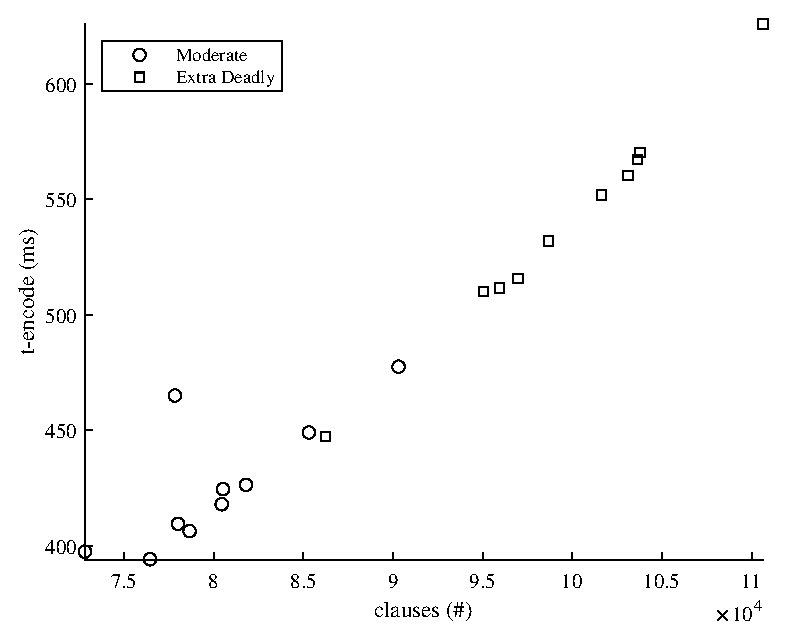
\includegraphics[width = 0.85\textwidth]{Figures/killer_BDD_encode.eps}
    \caption{Encoding time per clause, using Binary Decision Diagrams}
    \label{killerBDDencode}
\end{figure}
\begin{figure}
    \centering
    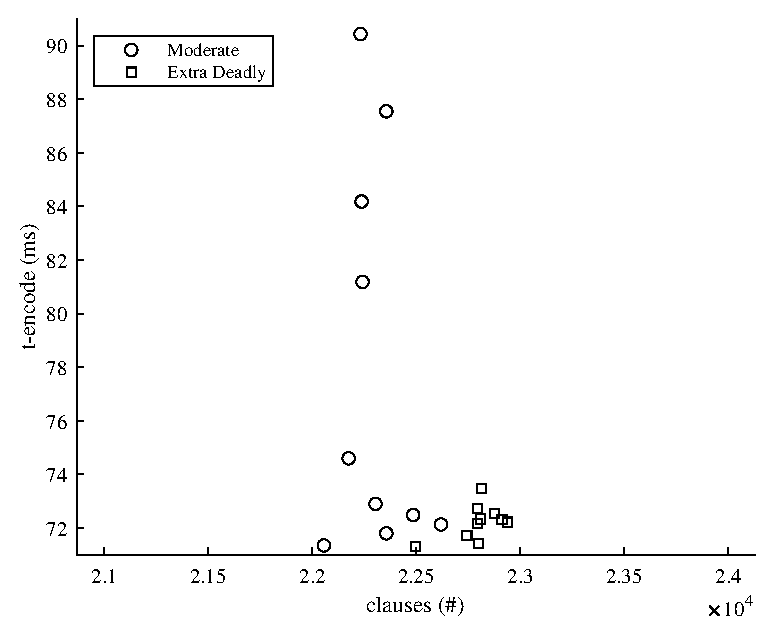
\includegraphics[width = 0.85\textwidth]{Figures/killer_AN_encode.eps}
    \caption{Average encoding time per clause, using Adder Networks}
    \label{killerANencode}
\end{figure}

\begin{figure}
    \centering
    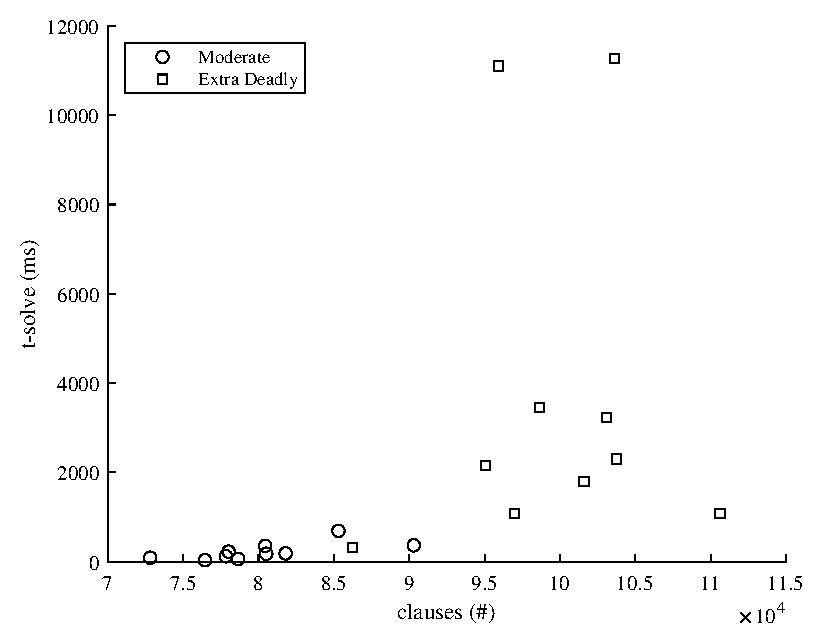
\includegraphics[width = 0.85\textwidth]{Figures/killer_BDD_solve.eps}
    \caption{Average solving time per clause, using Binary Decision Diagrams}
    \label{killerBDDsolve}
\end{figure}

\begin{figure}
    \centering
    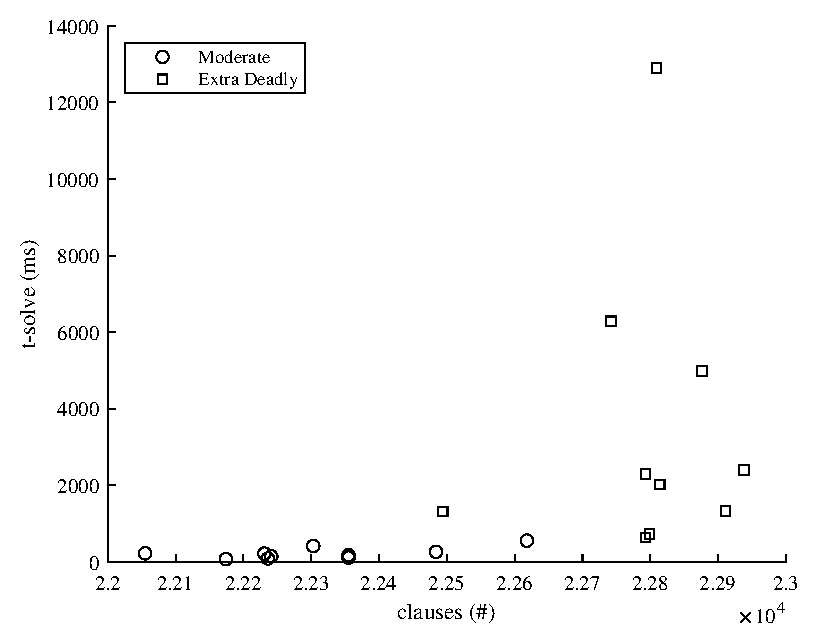
\includegraphics[width = 0.85\textwidth]{Figures/killer_AN_solve.eps}
    \caption{Average solving time per clause, using Adder Networks}
    \label{killerANsolve}
\end{figure}

\begin{figure}
    \centering
    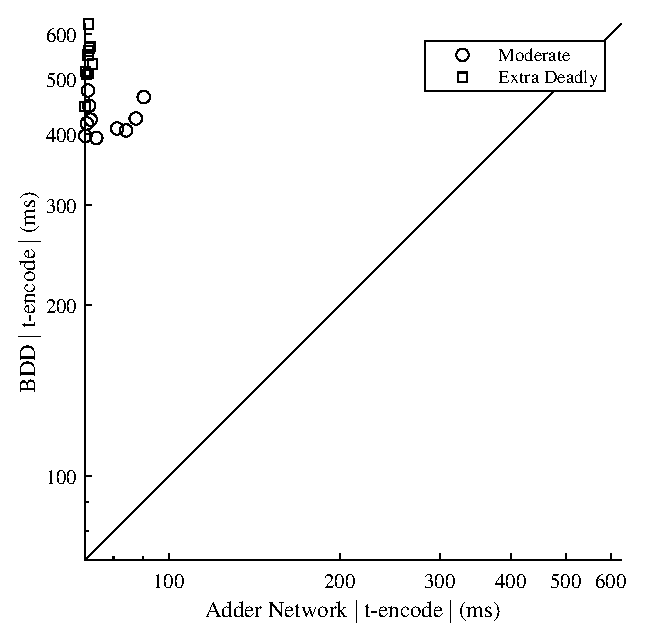
\includegraphics[width = 0.85\textwidth]{Figures/killer_encode_compare.eps}
    \caption{Average encoding time comparison, Binary Decision Diagrams vs. Adder Networks}
    \label{killerCompareEncode}
\end{figure}

\begin{figure}
    \centering
    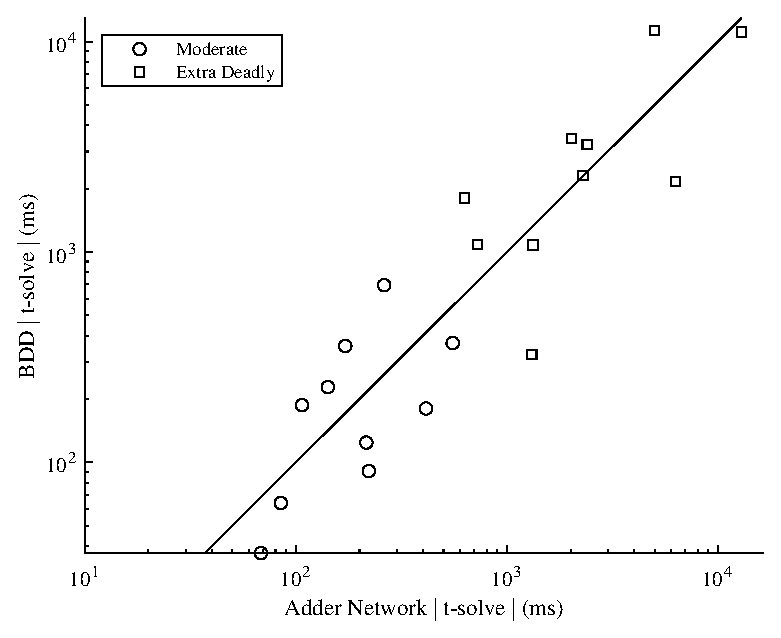
\includegraphics[width = 0.85\textwidth]{Figures/killer_solve_compare.eps}
    \caption{Average solving time comparison, Binary Decision Diagrams vs. Adder Networks}
    \label{killerCompareSolve}
\end{figure}
}

{
\renewcommand{\figurename}{Plot}
\begin{figure}
    \centering
    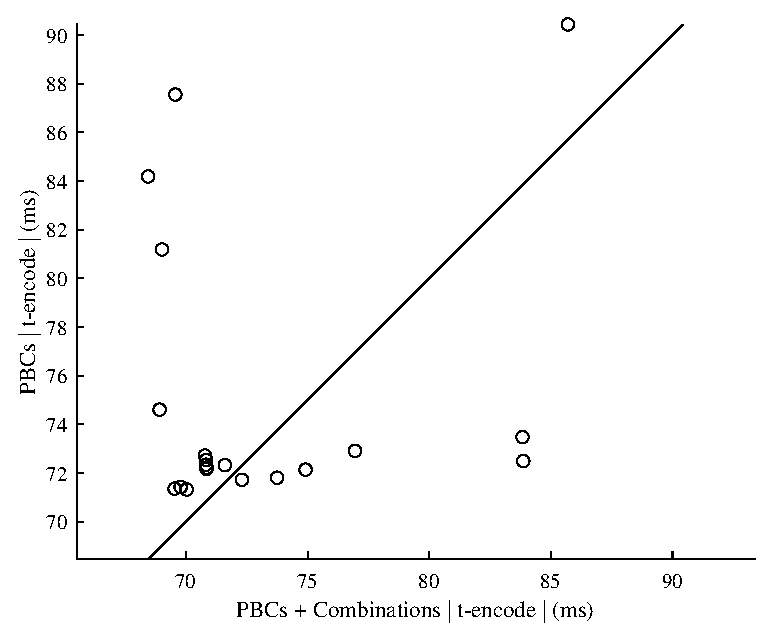
\includegraphics[width = 0.85\textwidth]{Figures/opt_encode_2_1.eps}
    \caption{Average encoding time comparison, PBCs vs. PBCs + Combinations}
    \label{opt_encode_2_1}
\end{figure}

\begin{figure}
    \centering
    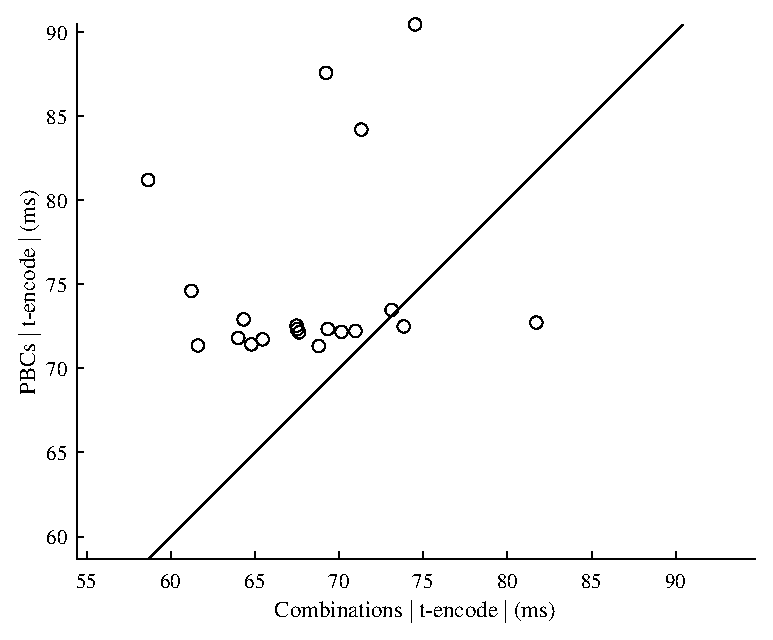
\includegraphics[width = 0.85\textwidth]{Figures/opt_encode_3_1.eps}
    \caption{Average encoding time comparison, PBCs vs. Combinations}
    \label{opt_encode_3_1}
\end{figure}

\begin{figure}
    \centering
    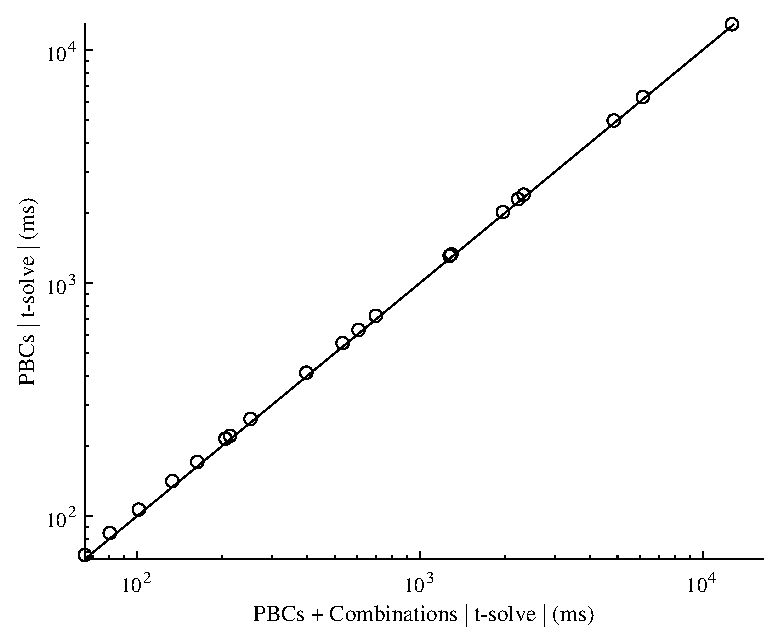
\includegraphics[width = 0.85\textwidth]{Figures/opt_solve_2_1.eps}
    \caption{Average solving time comparison, PBCs vs. PBCs + Combinations}
    \label{opt_solve_2_1}
\end{figure}

\begin{figure}
    \centering
    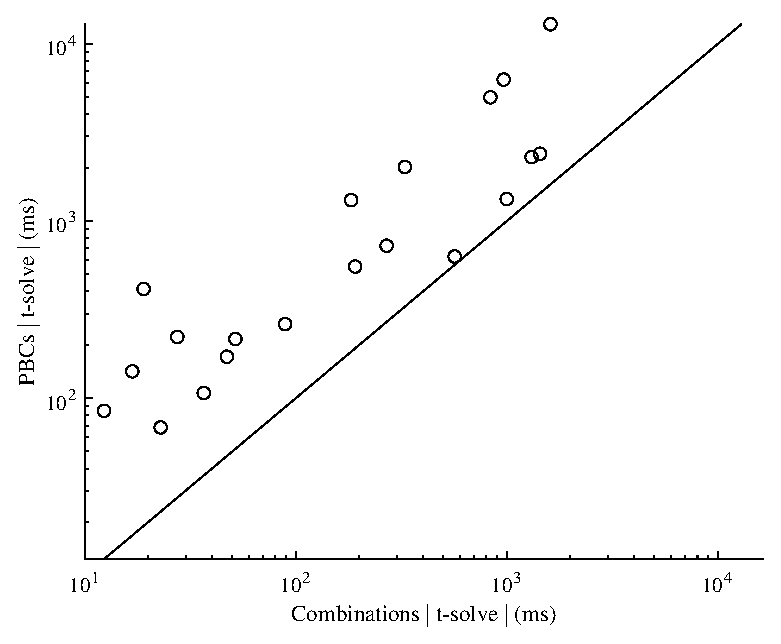
\includegraphics[width = 0.85\textwidth]{Figures/opt_solve_3_1.eps}
    \caption{Average solving time comparison, PBCs vs. Combinations}
    \label{opt_solve_3_1}
\end{figure}
}
\FloatBarrier

\begin{table}[t]
    \centering
    \renewcommand{\arraystretch}{1.5}
    \resizebox{\textwidth}{!}{
    \begin{tabular}{ |l|r|r|r|r|r|r|r|r|}
    \hline
    \multicolumn{1}{|c|}{\multirow{3}{*}{Variant}} & \multicolumn{3}{c|}{\makecell[c]{$t$-avg.\\(ms)}} & \multicolumn{3}{c|}{\makecell[c]{$t$-std.\\(ms)}} & \multicolumn{1}{c|}{\multirow{3}{*}{\#clauses}} & \multicolumn{1}{c|}{\multirow{3}{*}{\#variables}}\\\cline{2-7}
    & \multicolumn{1}{c|}{\multirow{2}{*}{encode}} & \multicolumn{2}{c|}{\makecell[c]{solve}} & \multicolumn{1}{c|}{\multirow{2}{*}{encode}} & \multicolumn{2}{c|}{\makecell[c]{solve}} &&\\\cline{3-4}\cline{6-7}
    && \makecell[c]{Sat4j} & \makecell[c]{MiniSat} & & \makecell[c]{Sat4j} & \makecell[c]{MiniSat} &&\\
    \hline
    9 Marks The Spot        &4428.02       & 170.90       &     1179.53      &211.03        & 36.76        &        519.18    & 727636 & 5994\\
    \hline
    Chess Sudoku            & 29.05       & 3.23        &      1061.05     &       1.10   &       0.43   &       241.94     &  8912 & 729\\
    \hline
    Fawlty Towers           & 65.38      &     11.10    &         904.62   &   12.31      &    0.71     &         127.42   & 17632& 2186 \\
    \hline
    Frozen Picnic           & 168.32      &    14.92    &         886.33   &    3.99      &      0.81    &         51.47   & 40519 & 5387\\
    \hline
    Mark 1                  &  28.60       &   8.18       &     903.05       &    2.12     &    0.50      &        52.05     &8839 & 729\\
        \hline
    Nurikabe Sudoku         & 77406.68      &        4145268.40       &          413259.82          &        3341.18       &        536495.31       &          5633.74         & 13904145 & 1169013\\
    \hline
    Sudoku Man Of Mystery   & 23.18        &     1.97     &      876.67      &   0.93       &  0.71        &         6.85     &  7399 & 729\\
    \hline
    The Miracle Thermo      & 739.77       &    446.32    &        1671.62   &    261.78   &     24.74    &        112.12    & 138743 & 5265\\
    \hline
    The Original Sandwich   &   1677.18    &    15408.00  &       2059.25    &    26.28    &   384.06    &       12.22     & 302640 & 42635\\
    \hline
    The Pyramid             &    48.68     &    219.07    &         1434.53  &    2.23      &    3.46    &         3.36     &15233& 1679\\
    \hline
    Thermo 2020             &  24.23       &     1.97    &         1355.67  &   1.09       &      0.66   &       54.23      & 7659 & 729\\
    \hline
    Thermo Couples          &  27.98       &    3.80      &          1354.52 &     0.85   &     0.55     &        8.19      & 8884 & 729\\
    \hline
    Thermo Squares          & 23.92        &    17.95     &        1362.25   &    0.74      &      0.67    &          54.87   & 7692 & 729\\
    \hline
    The Road To Genius      &   22.95       &    1.97      &      1364.20     &    0.81    &     0.74     &          56.83   &  7401 & 729\\
    \hline
    \end{tabular}
    }
    \renewcommand{\arraystretch}{1}
    
    \captionsetup{justification=centering,margin=2cm}
    \caption{CTCGH Sudokus, solving with Sat4j and MiniSat, \\PBC-Encoding with Adder Networks}
    
    \label{Experimnet:CTCGH}
\end{table}



\begin{table}[t]
    \renewcommand{\arraystretch}{1.5}
    \centering
    \resizebox{0.6\textwidth}{!}{
    
    \begin{tabularx}{30.56em}{|l|c|c|c|c|c|c|c|c|c|}
    \hline
    \multicolumn{1}{|c|}{\multirow{1}{*}{
     \belowbaseline[0ex]{~~~\rotatebox{45}{\parbox{3cm}{\raggedright{~Instance $\vert$ Rule}}}}}} &
     \belowbaseline[0ex]{\rotatebox{90}{\parbox{2.8cm}{\raggedright{~Normal Sudoku}}}} &
     \belowbaseline[0ex]{\rotatebox{90}{\parbox{2.8cm}{\raggedright{~Anti-Knight}}}} &
     \belowbaseline[0ex]{\rotatebox{90}{\parbox{2.8cm}{\raggedright{~Killer Sudoku}}}} &
     \belowbaseline[0ex]{\rotatebox{90}{\parbox{2.8cm}{\raggedright{~Arrowheads}}}} &
     \belowbaseline[0ex]{\rotatebox{90}{\parbox{2.8cm}{\raggedright{~Thermometers}}}} &
     \belowbaseline[0ex]{\rotatebox{90}{\parbox{2.8cm}{\raggedright{~Sandwich Sum}}}} &
     \belowbaseline[0ex]{\rotatebox{90}{\parbox{2.8cm}{\raggedright{~Secret Direction}}}} &
     \belowbaseline[0ex]{\rotatebox{90}{\parbox{2.8cm}{\raggedright{~Fawlty Towers}}}} &
     \belowbaseline[0ex]{\rotatebox{90}{\parbox{2.8cm}{\raggedright{~Nurikabe Sudoku}}}}\\
    \hline 
    9 Marks The Spot & $\times$& & & & & & $\times$& & \\
    \hline 
    Chess Sudoku &$\times$ & $\times$& & & $\times$& & & & \\ 
    \hline 
    Fawlty Towers &$\times$ & & & & & & &$\times$ & \\
    \hline 
    Frozen Picnic &$\times$ & & &$\times$ &$\times$ &$\times$ & & & \\
    \hline 
    Mark 1 &$\times$ &$\times$ & & & $\times$& & & & \\
    \hline 
    Nurikabe Sudoku & $\times$& & & & & & & & $\times$\\
    \hline 
    Sudoku Man Of Mystery & $\times$& & & & & & & & \\
    \hline 
    The Miracle Thermo &$\times$ & & & &$\times$ & & & & \\
    \hline 
    The Original Sandwich & $\times$& & & & &$\times$ & & & \\
    \hline 
    The Pyramid &$\times$ &$\times$ & $\times$& & & & & & \\
    \hline 
    Thermo 2020 & $\times$& & & &$\times$ & & & & \\
    \hline 
    Thermo Couples & $\times$&$\times$ & & &$\times$ & & & & \\
    \hline 
    Thermo Squares &$\times$ & & & & $\times$& & & & \\ 
    \hline 
    The Road To Genius &$\times$ & & & & & & & & \\ 
    \hline
    \end{tabularx}
    }
    \renewcommand{\arraystretch}{1}
    \caption{Sudoku Puzzle Instances and their rules.}
    \label{tab:InstanceRule}
\end{table}


% !TEX root = ../Thesis.tex
\chapter{Conclusion}
This thesis demonstrated how different variants and rules of Sudoku Puzzles could be encoded as sets of logical clauses. We have seen that in most cases, SAT-solvers can find assignments that satisfy these sets of clauses in a relatively short time. We also found that solving Sudokus is by no means a trivial problem as the number of clauses and the time needed to solve ``Nurikabe Sudoku'' have shown. We have elaborated in detail on how Pseudo Boolean Constraints can be used to encode constraints regarding sums, like in Killer Sudokus or for the Sandwich-Sum rules. Specifically for Killer Sudoku instances, we found that both shown encoding methods Adder Networks and Binary Decision Diagrams (both proposed by \cite{Een2006TranslatingPC}) have comparable performance, but that Adder Networks produce fewer clauses and are encoding the PBCs faster. Additionally, we have shown that encoding Killer Sudokus without PBCs can significantly reduce the time needed to solve them.\\
\\
In future work, the proposed encoding methods for Sudoku rules could help to craft new puzzle instances of exotic Variants like ``9 Marks The Spot'' or ``The Miracle Thermo''. Further, we came across multiple engaging questions for which we only estimated an answer or gave an upper bound, like what is the highest possible number of islands in ``Nurikabe Sudoku" or how long can a hidden path in ``9 Marks The Spot'' be at maximum. Also teasing: CTCGH \cite{CrackingTheCryptic2021} contains many more Sudoku variants which could be analysed and encoded for SAT-Solvers.\\
\\
During our work, we only used a limited test set of puzzle instances, which all had to be rewritten by hand into a format our program could understand. In general, there seem to be no common test sets for non-original Sudoku Variants like Killer Sudoku, which may also has to do with the lack of a common file format that could be used to share more exotic Puzzle variants. To facilitate future work, it would be desirable to agree on a standard file format specifically tailored for Sudokus. This would allow the puzzle and research community to build an openly available and directly usable database of Sudoku Puzzles, which would make the testing and analysis of new encoding and solving algorithms more reliable.
%\input{./Chapters/Chapter7}
%% ----------------------------------------------------------------
\thesisappendix
\thesisbib
\begin{appendices}
	% !TEX root = ../Thesis.tex
\chapter{Appendix} 
\end{appendices}
%% ----------------------------------------------------------------
\thesisback
\iflanguage{english}
  {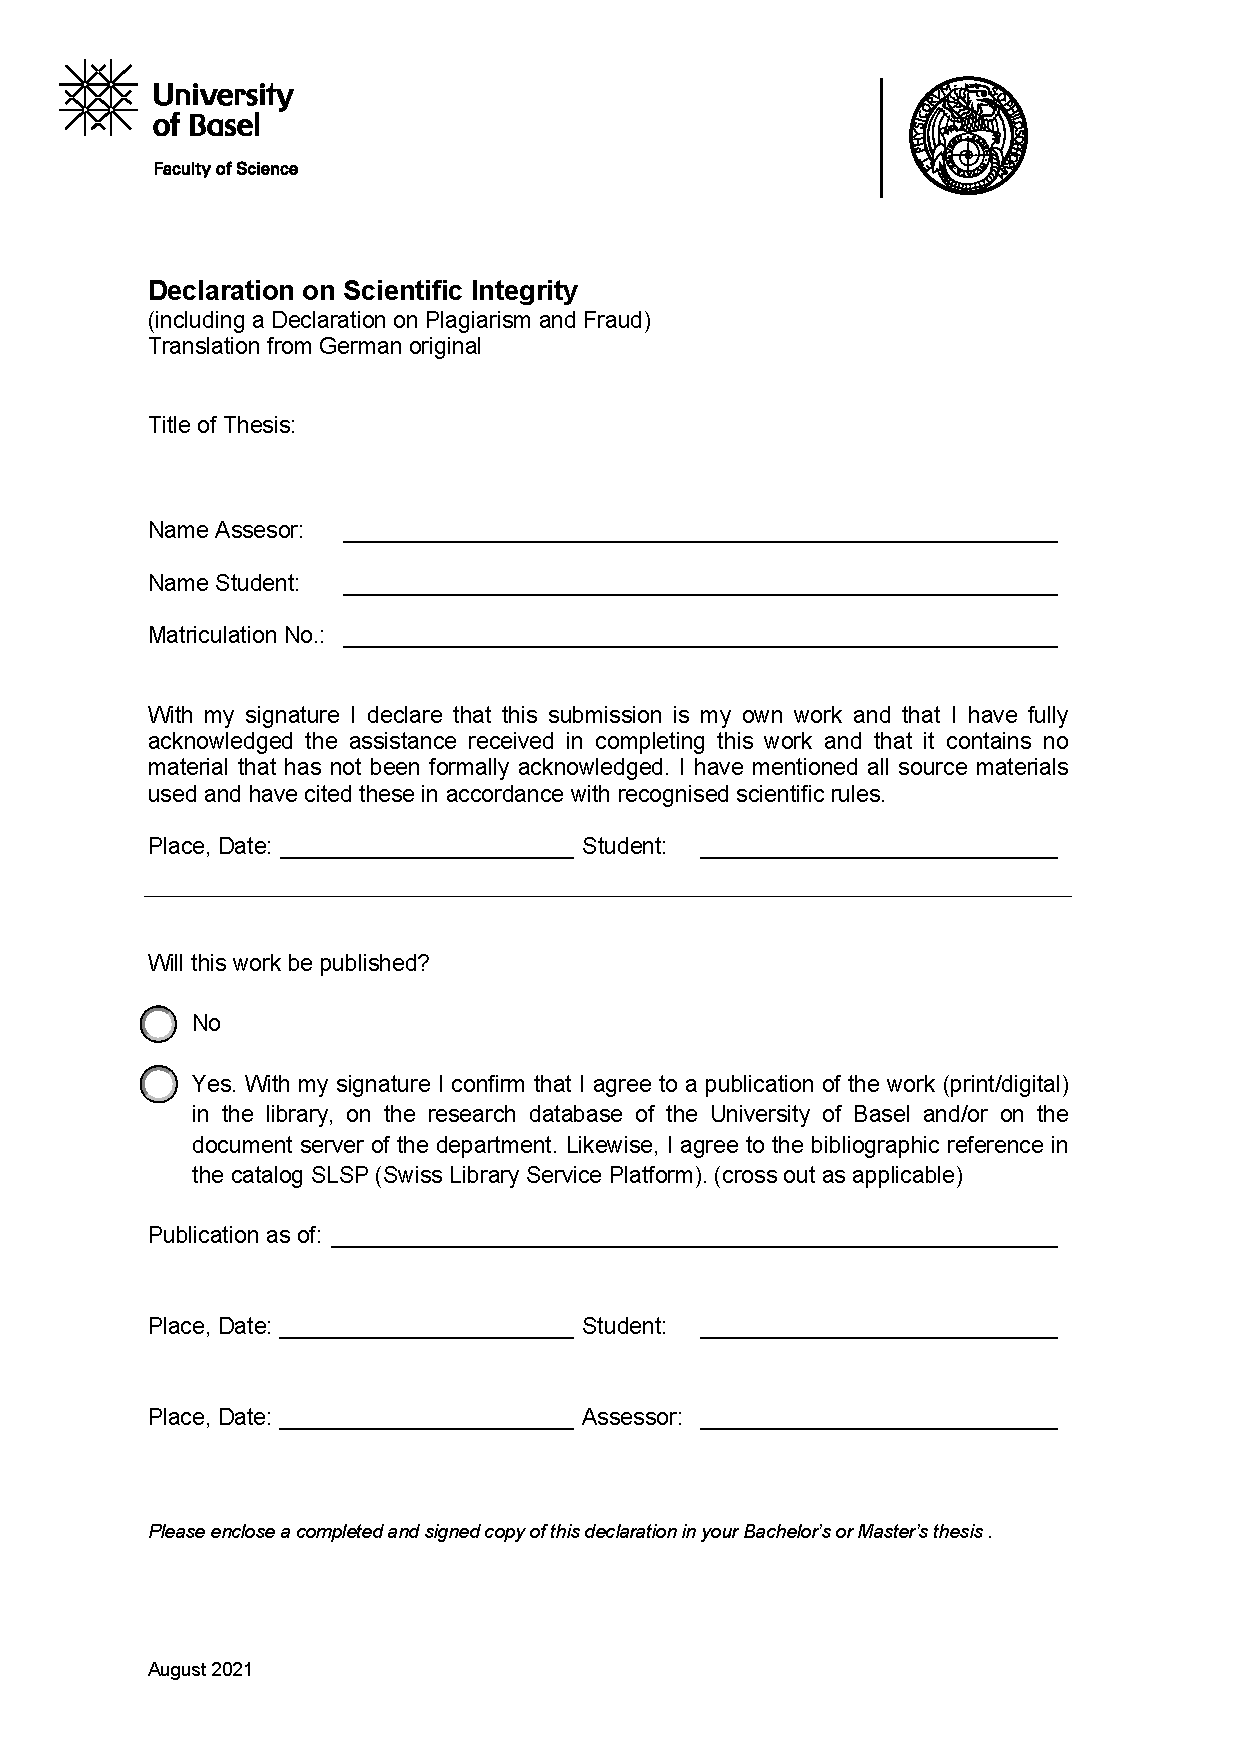
\includepdf{./Back/wissensch_Redlichkeit_E_Aug_21.pdf}}
  {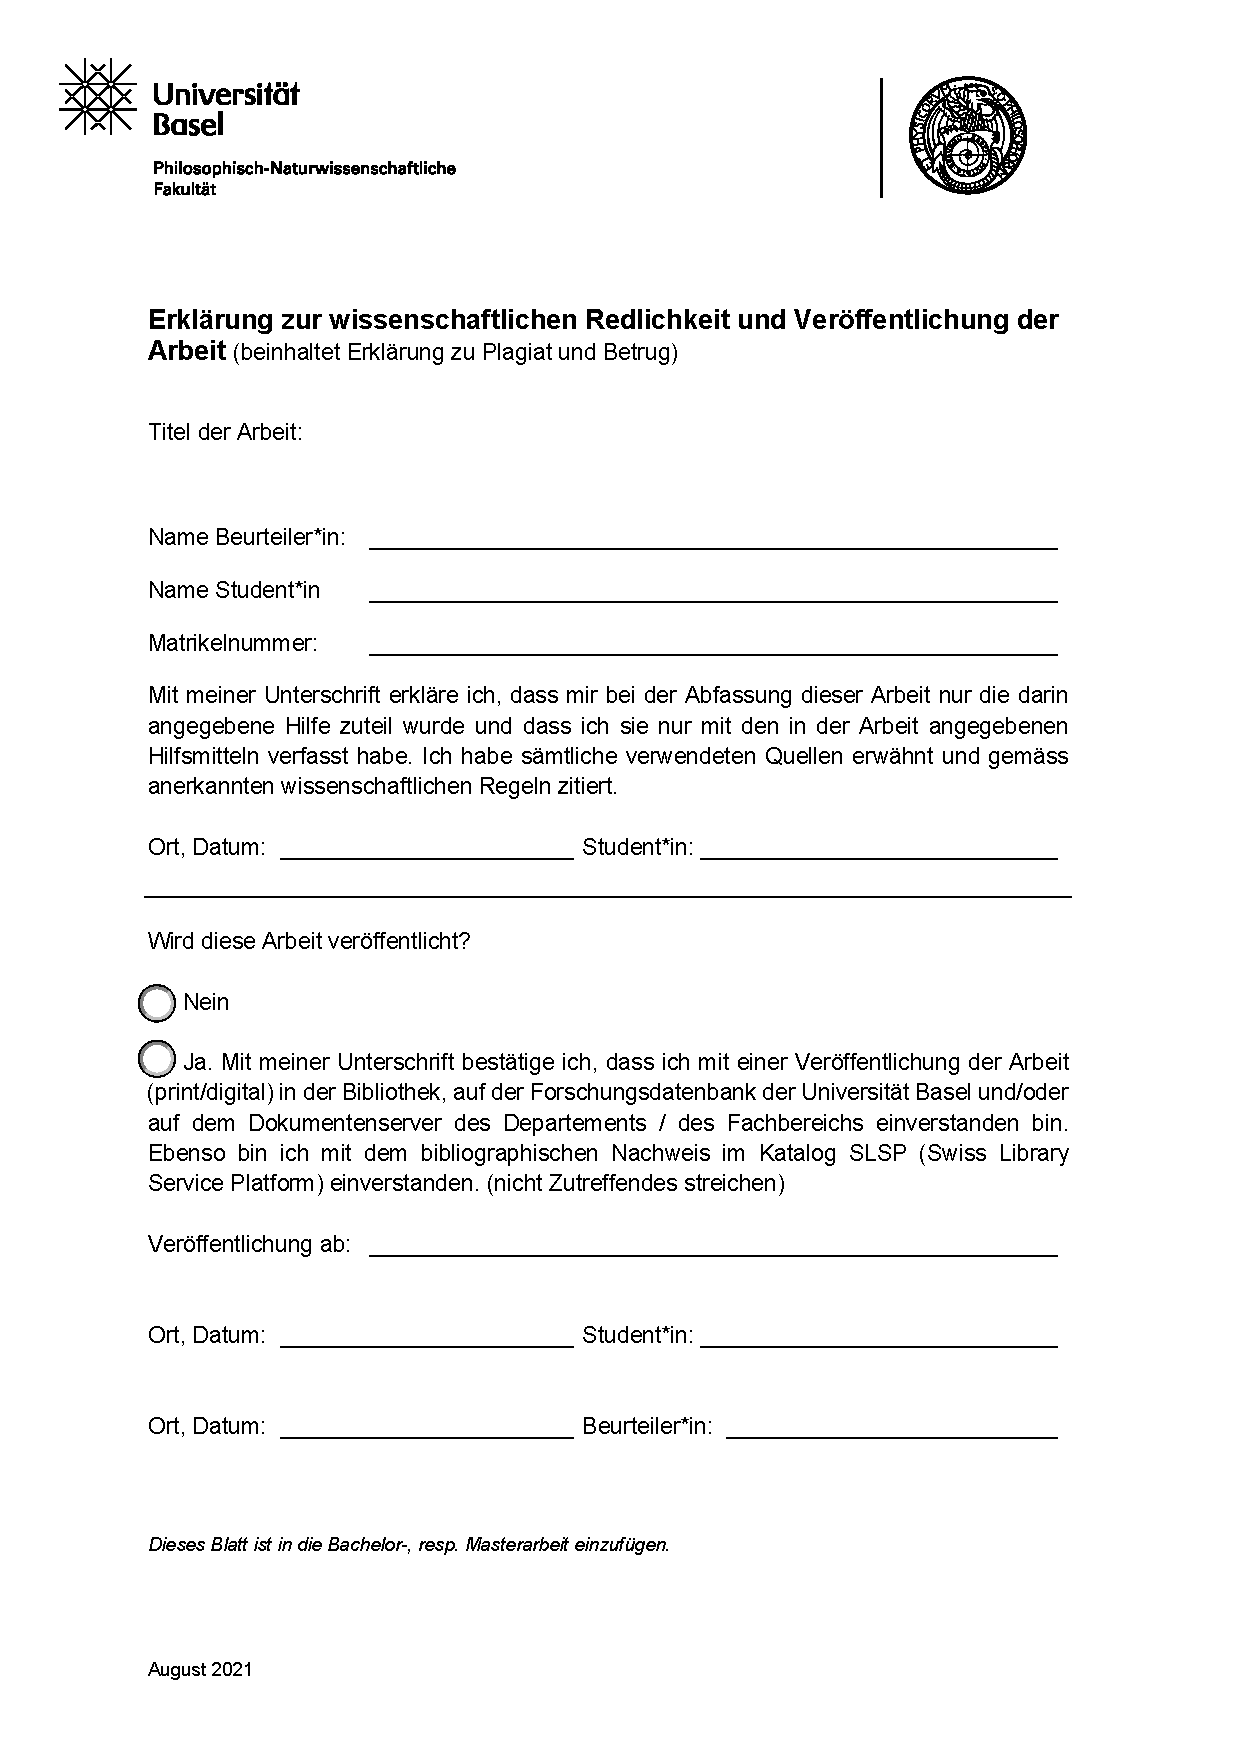
\includepdf{./Back/wissensch_Redlichkeit_D_Aug_21.pdf}}
%% ----------------------------------------------------------------
\end{document}
%% ----------------------------------------------------------------
